\documentclass[11pt,a4paper]{article}

% ============================================================
% PAQUETES (mismo preambulo que e1_informe/informe_e1_smnv3.tex)
% ============================================================
\usepackage[utf8]{inputenc}
\usepackage[T1]{fontenc}
\usepackage[spanish,es-nodecimaldot]{babel} % es-nodecimaldot: punto decimal también en modo matemático
\usepackage{geometry}
\geometry{a4paper,margin=2.3cm}
\usepackage{booktabs}
\usepackage{array}
\usepackage{graphicx}
\usepackage{adjustbox}
\usepackage{caption}
\usepackage{float}
\usepackage{fancyhdr}
\usepackage{xcolor}
\usepackage{hyperref}
\usepackage{enumitem}
\usepackage{natbib}
\usepackage{amsmath}
\usepackage{amssymb}


\hypersetup{
  colorlinks=true,
  linkcolor=blue!50!black,
  urlcolor=blue!60!black,
  citecolor=blue!50!black,
  pdftitle={Informe tecnico -- Entregable 3 -- Proyecciones de la TSM y del ENOS en Nino 3.4 / Nino 1+2},
  pdfauthor={Jonathan Paredes}
}

% \archivo{...}: rutas/nombres de archivo en monoespaciada con corte de
% linea en guiones bajos (igual que en el informe del E1). Usar con
% guion bajo LITERAL dentro del argumento.
\urlstyle{tt}
\newcommand{\archivo}[1]{\begingroup\hypersetup{urlcolor=black}\url{#1}\endgroup}
\newcolumntype{L}[1]{>{\raggedright\arraybackslash}p{#1}}

\captionsetup{font=small,labelfont=bf}

\pagestyle{fancy}
\fancyhf{}
\fancyhead[L]{\small Entregable N°3 -- Influencia del cambio climático en los eventos de El Niño y sus impactos en el Perú}
\fancyhead[R]{\small \thepage}
\renewcommand{\headrulewidth}{0.4pt}

\setlength{\parskip}{0.4em}
\setlength{\parindent}{1.2em}

\begin{document}
\selectlanguage{spanish}

% ============================================================
% PORTADA (mismo formato que el Entregable 1)
% ============================================================
\begin{titlepage}
\centering
\noindent\rule{\textwidth}{0.6pt}

\vspace{1.2cm}
{\Large \bfseries ENTREGABLE N\textsuperscript{o}~3 \par}
\vspace{1.2cm}
\rule{0.7\textwidth}{0.6pt}

\vspace{1.2cm}
{\normalsize \bfseries Concepto: \par}
\vspace{0.3cm}
{\large \bfseries Servicio de asistencia en temas de investigación para evaluar\\
la influencia del cambio climático en los eventos de El Niño\\
y sus impactos en el Perú \par}

\vspace{1.4cm}
{\small Servicio prestado para el SENAMHI \par}

\vspace{1.4cm}
{\normalsize \bfseries Actividad: \par}
\vspace{0.2cm}
{\normalsize Tercer entregable - Informe del desarrollo de la actividad c)\\
indicada en el numeral 6 del TDR \par}

\vspace{1.2cm}
\rule{0.7\textwidth}{0.6pt}

\vspace{0.3cm}
{\small \bfseries Responsable: \par}
\vspace{0.2cm}
{\small Ing. Jonathan Aaron Paredes Quispe \par}
\vspace{0.3cm}
\rule{0.7\textwidth}{0.6pt}

\vfill
{\small \bfseries FECHA: \today \par}
\vspace{0.6cm}
\noindent\rule{\textwidth}{0.6pt}
\end{titlepage}

\tableofcontents
\listoffigures
\listoftables
\clearpage

% ============================================================
\section{Resumen}
% ============================================================

Este informe documenta el Entregable~3 del servicio de asistencia en temas de investigación de SENAMHI sobre la influencia del cambio climático en El Niño-Oscilación del Sur (ENOS). Analiza cómo cambian la temperatura superficial del mar (TSM) y el ENOS en las regiones Niño~3.4 y Niño~1+2 en dos periodos futuros, 2036--2065 (P1) y 2071--2100 (P2), frente a 1985--2014 (ref), bajo tres escenarios de emisiones: SSP2-4.5, SSP3-7.0 y SSP5-8.5. Se usan los 15 modelos CMIP6 seleccionados en el Entregable~2, con los 40 como contraste. Cada modelo se compara con su propio pasado, de modo que su error fijo se cancela, y los resultados se resumen con la mediana de los modelos, su acuerdo de signo y una prueba de significancia con corrección por pruebas múltiples.

\textbf{Estado medio.} El calentamiento es el resultado más firme: todos los modelos lo proyectan en todos los escenarios. En P2, Niño~3.4 se calienta $+1.9$, $+2.6$ y $+3.4$\,°C y Niño~1+2 $+2.3$, $+2.8$ y $+3.6$\,°C bajo SSP2-4.5, SSP3-7.0 y SSP5-8.5. Niño~1+2 se calienta además entre 0.4 y 0.7\,°C más que el promedio del trópico, con acuerdo de los 15 modelos.

\textbf{Variabilidad.} La variabilidad del ENOS ($\sigma_{3m}$, ver glosario: qué tan intensos son los Niños y las Niñas típicos) tiende a aumentar en Niño~3.4: $+11$, $+23$ y $+26$\,\% en la mediana en P2, pero los modelos discrepan mucho (de $-29$ a $+105$\,\% con SSP5-8.5) y el cambio no es robusto. En Niño~1+2 el cambio es pequeño ($+2$ a $+9$\,\%) y sin acuerdo.

\textbf{Ocurrencia de eventos extremos.} Los eventos fuertes o más intensos del ONI y del RONI aumentan de forma significativa: pasan de 3 a entre 5 y 9 por cada 30 años con SSP3-7.0 y SSP5-8.5. La frecuencia total de eventos cálidos sube entre 11 y 44\,\% en la mediana (por ejemplo, el ONI pasa de 8 a 10--11 eventos cada 30 años), pero casi nunca de forma significativa: con unos 9 eventos por periodo la señal no se distingue del azar. Medido contra el clima actual (base fija), a fin de siglo la TSM de Niño~1+2 pasa casi todo el tiempo por encima del umbral de El Niño de hoy, por el calentamiento de fondo y no por un ENOS más activo.

\begin{table}[H]
\caption{Glosario de términos, símbolos y acrónimos del informe.}
\label{tab:glosario}
\centering
\scriptsize
\renewcommand{\arraystretch}{1.05}
\setlength{\tabcolsep}{3pt}
\begin{tabular}{@{}L{2.0cm}L{\dimexpr0.5\textwidth-2.0cm-5\tabcolsep\relax}|L{2.0cm}L{\dimexpr0.5\textwidth-2.0cm-5\tabcolsep\relax}@{}}
\toprule
\textbf{Término} & \textbf{Significado} & \textbf{Término} & \textbf{Significado} \\
\midrule
TSM & Temperatura superficial del mar. & ONI & Índice Oceánico El Niño (NOAA): anomalía de TSM de Niño~3.4, media de 3 meses, base móvil. \\
ENOS & El Niño-Oscilación del Sur: El Niño (fase cálida) y La Niña (fría). & RONI & ONI relativo: ONI menos la anomalía del trópico, reescalado. \\
Niño~3.4 / Niño~1+2 & Pacífico central (5°S--5°N, 170°--120°W) / costa de Perú y Ecuador (10°S--0°, 90°--80°W). & ICEN & Índice Costero El Niño (ENFEN): anomalía de TSM de Niño~1+2, media de 3 meses. \\
CMIP6 & Proyecto de intercomparación de modelos climáticos, fase 6. & ONIfija, ICENfija & ONI e ICEN con base fija 1985--2014. \\
SSP2-4.5 / 3-7.0 / 5-8.5 & Escenarios de emisiones intermedias, altas y muy altas. & Base móvil / fija & Clima ``normal'' que se actualiza cada 5 años / fijo en 1985--2014. \\
ref, P1, P2 & 1985--2014; 2036--2065; 2071--2100 (30 años cada uno). & Evento cálido & ONI $\geq 0.5$\,°C en 5 trimestres seguidos; ICEN $> 0.5$\,°C en 3 meses seguidos. \\
Anomalía & TSM menos su valor normal de ese mes (climatología mensual). & Evento fuerte o más & ONI $\geq 1.5$\,°C; ICEN $> 2.1$\,°C (ENFEN, 2024). \\
$\Delta$TSM & TSM media de P1 o P2 menos la de ref, en cada modelo. & ev/30 años & Eventos en un periodo de 30 años, el largo de ref, P1 y P2. \\
Cambio relativo & $\Delta$TSM de la caja menos $\Delta$TSM del trópico (20°S--20°N). & Razón de frecuencias & Frecuencia en P entre la de ref: 1 = sin cambio; 1.25 = 25\,\% más. \\
$\sigma$ & Desviación estándar de la anomalía sin tendencia. & Mediana, p10--p90 & Valor central de los modelos y rango del 80\,\% central. \\
$\sigma_{3m}$ & $\sigma$ de la anomalía suavizada a 3 meses (la serie del ONI y del ICEN): intensidad de los Niños y Niñas típicos. & Acuerdo de signo & Fracción de modelos con el signo de la mediana; $\geq 0.8$ = robusto (IPCC). \\
$\Delta\sigma_{3m}$ & Cambio de $\sigma_{3m}$ en \%: $100(\sigma_{3m,P}/\sigma_{3m,\mathrm{ref}}-1)$. & Significativo ($^{*}$) & No atribuible al azar: Wilcoxon con corrección de Holm, $p<0.05$. \\
TdR & Términos de Referencia del servicio. & Conjuntos 15, 40, 11, 7 & Selección del E2; todos; los 15 sin los 4 de ICEN más débil; los 7 con mejor evento típico. \\
\bottomrule
\end{tabular}
\end{table}

\clearpage
% ============================================================
\section{Alcance}
\label{sec:alcance}
% ============================================================

Los Términos de Referencia del servicio (en adelante, \textsc{TdR}) definen el Entregable~3 como la actividad~(c): analizar las proyecciones futuras de la TSM y de la variabilidad del ENOS en las regiones Niño~3.4 y Niño~1+2, y evaluar la influencia del cambio climático sobre el estado medio, la variabilidad y la ocurrencia de eventos extremos mediante índices como el ONI y el ICEN. Los resultados responden a esos tres puntos: el estado medio (Sección~\ref{sec:res_media}), la variabilidad (Sección~\ref{sec:res_var}) y la ocurrencia de eventos, con el tiempo sobre el umbral de El Niño (Sección~\ref{sec:res_umbral}) y la frecuencia, la intensidad y los eventos extremos (Sección~\ref{sec:res_eventos}). La Sección~\ref{sec:res_sintesis} reúne las respuestas en un solo cuadro. Los análisis que ayudan a interpretar, pero que el TdR no pide (el mapa del patrón relativo al trópico, el ciclo anual, la variabilidad por estación, la asimetría, el tipo de evento, el espectro y la sensibilidad al conjunto de modelos), están en el Anexo (Sección~\ref{sec:anexo}). Además de los escenarios SSP2-4.5 y SSP5-8.5 que indica el TdR, se usa también SSP3-7.0.

El insumo son los productos de los entregables anteriores: la TSM de los 40 modelos en la grilla común del Entregable~1 (\archivo{data/processed/masked/}) y, del Entregable~2, la selección de 15 modelos con su \emph{skill score}, la construcción de los índices ONI, RONI e ICEN, los criterios de detección y clasificación de eventos cálidos, las tres pruebas del filtro de eventos (frecuencia, duración y estacionalidad) y su recomendación de comparar conjuntos de modelos. Lo que agrega este entregable es su aplicación al futuro: el cambio de cada modelo entre periodos de 30 años, el cambio relativo al trópico, el RONI con el factor de escala calculado solo en la base y dos índices de base fija (ONIfija e ICENfija), las pruebas del filtro aplicadas entre periodos del mismo modelo en lugar de frente a ERSSTv5, los conjuntos de 11 y 7 modelos y la significancia del cambio multimodelo (Wilcoxon con corrección de Holm). Este entregable no descarga datos ni corrige sesgos. La partición de la incertidumbre (variabilidad interna, modelos y escenarios), la relación señal-ruido y el tiempo de emergencia corresponden al Entregable~4.



% ============================================================
\section{Marco metodológico}
\label{sec:metodo}
% ============================================================

Esta sección define cada métrica y cada prueba estadística del Entregable~3 tal como se implementaron en \archivo{scripts_e3/} (pasos q01--q11). Cada estadístico se presenta en dos niveles: primero, en lenguaje simple, qué dato entra, qué se hace con él y por qué se hace de esa forma; después, una \textbf{Definición formal}, breve, con la ecuación tal como está implementada y sus supuestos.
Los ejemplos numéricos usan AWI-CM-1-1-MR (M03), el primer modelo de la selección del Entregable~2, bajo SSP5-8.5. Los términos y símbolos que se repiten están en el glosario (Cuadro~\ref{tab:glosario}), después del Resumen.


% ------------------------------------------------------------
\subsection{Conceptos básicos de las pruebas estadísticas}
\label{sec:conceptos}

Una prueba estadística responde si una diferencia observada es \emph{real} o podría deberse al azar. Por ejemplo, si un modelo produce 8 Niños en 1985--2014 y 12 en 2036--2065, ¿aumentaron los Niños o fue la suerte de esos 30 años? Aun sin ningún cambio en el clima, dos periodos de 30 años nunca dan exactamente el mismo número de eventos, igual que lanzar una moneda 30 veces no da siempre 15 caras.

La prueba parte de suponer que \emph{no hay cambio} (la ``hipótesis nula'') y calcula qué tan raro sería, bajo ese supuesto, ver una diferencia tan grande como la observada. Esa probabilidad es el \textbf{valor $p$}. Si es muy pequeña (por convención, menor que 5\,\%, es decir, $p < 0.05$), la diferencia es difícil de explicar por azar y se dice que el cambio es \textbf{estadísticamente significativo}. Si $p$ es grande, no se puede descartar el azar, lo que \emph{no} es lo mismo que demostrar que no hubo cambio: puede que los datos sean muy pocos para verlo. La capacidad de una prueba para detectar un cambio que sí existe se llama \textbf{potencia}, y crece con la cantidad de datos.

Significativo tampoco quiere decir grande o importante: un cambio de 0.1\,°C puede ser significativo con muchos datos, y uno de 30\,\% puede no serlo con pocos. Por eso este informe reporta siempre la magnitud del cambio junto a su significancia.

\noindent\textbf{Definición formal.} Una prueba contrasta una hipótesis nula $H_0$ con una alternativa $H_1$ (aquí siempre bilateral) mediante un estadístico $T$ cuya distribución bajo $H_0$ es conocida, exacta, asintótica o por permutación. El valor $p$ es $\Pr(|T| \ge |t_{\mathrm{obs}}| \mid H_0)$. Se rechaza $H_0$ si $p < \alpha$, con $\alpha = 0.05$, lo que acota en $\alpha$ la probabilidad de un falso positivo (error de tipo I). La potencia es $1-\beta$, con $\beta$ la probabilidad de no rechazar $H_0$ cuando es falsa (error de tipo II). Cuando se hacen $k$ pruebas, la probabilidad de al menos un falso positivo crece hasta $1-(1-\alpha)^k$ si son independientes; se corrige con el método de Holm (Sección~\ref{sec:holm}).

% ------------------------------------------------------------
\subsection{Periodos, escenarios y conjuntos de modelos}
\label{sec:periodos}

Se comparan tres periodos de 30 años: la referencia 1985--2014 (en adelante, ref), el futuro cercano P1 = 2036--2065 y el futuro lejano P2 = 2071--2100, bajo tres escenarios de emisiones: SSP2-4.5 (intermedio), SSP3-7.0 (alto) y SSP5-8.5 (muy alto). Cada serie mensual concatena el experimento \texttt{historical} (hasta 2014-12) con el escenario (desde 2015-01). La referencia tiene 30 años, y no los 34 de la climatología del Entregable~2 (1981--2014), para que las desviaciones estándar, los conteos de eventos y los espectros de los tres periodos se estimen con muestras del mismo largo; 1985--2014 es además la base fija del RONI en el Entregable~2. Dos modelos terminan sus escenarios en 2099-12 (CAMS-CSM1-0 e IITM-ESM; en SSP3-7.0, IITM-ESM termina en 2098-12): su P2 tiene 29 años (28 en ese caso), y todas las métricas se calculan con los meses disponibles.

Del Entregable~2 se toman la selección de 15 modelos, el \emph{skill score} de cada modelo ($S_{\mathrm{final}}$ y $S_{\mathrm{ICEN}}$) y su recomendación (Sección~9 de ese informe): usar los 15 como conjunto principal y los 40 como contraste, y comprobar si la señal cambia al quitar los modelos de menor $S_{\mathrm{ICEN}}$ (M34, M35, M12 y M40) o al quedarse con los siete que cumplen $S_{\mathrm{final}} \geq 0.9$ y $S_{\mathrm{ICEN}} \geq 0.9$. En este informe esa recomendación se aplica como cuatro conjuntos de modelos, y todos los resultados se calculan para cada uno. Los cuatro responden a una misma pregunta: ¿la señal proyectada depende de qué modelos se usen?
\begin{itemize}[nosep]
\item \textbf{15 modelos} (conjunto principal): los que pasaron el filtro de eventos del Entregable~2, es decir, cuya frecuencia, duración y estacionalidad de eventos cálidos no se distinguen de las observadas.
\item \textbf{40 modelos} (contraste): todos los evaluados. Responde: ¿cambia el resultado si no se selecciona ningún modelo?
\item \textbf{11 modelos}: los 15 sin los cuatro que simulan el Niño costero más débil. En el Entregable~2, $S_{\mathrm{ICEN}}$ mide cuánto se parece el evento cálido típico del ICEN de un modelo al observado: vale 1 si tiene la misma forma y amplitud, y baja cuanto más débil o más fuerte es. Los cuatro con menor valor son MPI-ESM1-2-HR (M34, 0.45; su Niño costero típico tiene menos de la mitad de la amplitud observada), CNRM-CM6-1-HR (M12, 0.79), MPI-ESM1-2-LR (M35, 0.81) y UKESM1-0-LL (M40, 0.83). Responde: ¿cambia la señal en Niño~1+2 si se quitan los modelos con Niños costeros demasiado débiles?
\item \textbf{7 modelos}: los que, además de pasar el filtro, tienen $S_{\mathrm{final}} \geq 0.9$ y $S_{\mathrm{ICEN}} \geq 0.9$, es decir, un evento típico bien representado tanto en Niño~3.4 como en Niño~1+2 (amplitud entre 28\,\% menor y 39\,\% mayor que la observada). Son AWI-CM-1-1-MR, ACCESS-ESM1-5, EC-Earth3, IITM-ESM, GFDL-ESM4, NorESM2-LM y CESM2. Responde: ¿cambia la señal si solo se usan los mejores?
\end{itemize}
El Entregable~2 no establece cómo comparar los conjuntos; en este informe se comparan por su mediana y su acuerdo de signo (Sección~\ref{sec:multimodelo}): si se mantienen en los cuatro, la conclusión no depende de la selección (Anexo, Figura~\ref{fig:a_sensibilidad}). La significancia (Wilcoxon con corrección de Holm) se interpreta sobre todo en el conjunto de 15, porque con 11 y 7 modelos la prueba casi no puede alcanzar valores $p$ pequeños.

% ------------------------------------------------------------
\subsection{Cambio del estado medio}
\label{sec:delta}

\textbf{Dato:} la TSM mensual de cada modelo, promediada en la caja Niño~3.4 o Niño~1+2. \textbf{Qué se hace:} se promedian los 360 meses de la referencia y los 360 del periodo futuro, y se restan. En M03, Niño~3.4 pasa de 25.61\,°C a 28.30\,°C en P2: un cambio de $+2.69$\,°C.

\textbf{Por qué así:} el Entregable~2 mostró que los modelos tienen errores fijos; casi todos son demasiado cálidos en Niño~1+2. Si se comparara el futuro de un modelo con la observación actual, ese error se confundiría con calentamiento. Comparando cada modelo \emph{con su propio pasado}, el error se resta y queda solo el cambio.

\textbf{Cambio relativo:} como todo el océano tropical se calienta, también se calcula cuánto \emph{más} (o menos) se calienta la caja que el promedio tropical. En M03, el trópico sube $+2.41$\,°C y Niño~1+2 $+3.22$\,°C: el cambio relativo de Niño~1+2 es $+0.81$\,°C. Un valor positivo significa que la costa norte del Perú se calienta más que el resto del trópico, un patrón ``tipo El Niño'' permanente.

\noindent\textbf{Definición formal.} Para el modelo $i$ y el periodo $P \in \{\mathrm{P1}, \mathrm{P2}\}$,
\begin{equation}
\label{eq:delta}
\Delta X_i = \overline{X}_{i,P} - \overline{X}_{i,\mathrm{ref}}, \qquad
\Delta X^{\mathrm{rel}}_i = \Delta X_{i,\mathrm{caja}} - \Delta X_{i,\mathrm{trop}},
\end{equation}
con la barra como media temporal del periodo y $X_{\mathrm{trop}}$ la media de 20°S--20°N ponderada por $\cos\phi$. El supuesto es que el sesgo de cada modelo es aproximadamente constante en el tiempo, el supuesto estándar de las proyecciones sin corrección de sesgo. $\Delta X^{\mathrm{rel}}$ mide el patrón del calentamiento \citep{xie2010}, con la misma idea con la que el RONI retira el calentamiento de fondo. En los mapas ambas cantidades se calculan punto a punto. La trayectoria de la Figura~\ref{fig:trayectoria} aplica la misma resta año a año: la media anual de cada año menos la media de 1985--2014 del mismo modelo, una base fija. No se usa la base móvil de 30 años que NOAA y el ENFEN actualizan cada 5 años, porque esa base sube con el calentamiento y lo retira de la anomalía: la curva quedaría cerca de 0 todo el siglo. La base móvil se usa solo en los índices ONI e ICEN, donde interesa medir el ENOS respecto del clima de su época (Sección~\ref{sec:indices}).

\textbf{Por qué el cambio relativo.} El cambio total de la TSM mezcla dos componentes: un calentamiento casi uniforme del trópico, cuya magnitud depende sobre todo de la sensibilidad climática de cada modelo, y un patrón espacial que se aparta de ese promedio. Siguiendo a \citet{xie2010} y \citet{ma2013}, el segundo se separa restando a cada punto el cambio medio de 20°S--20°N del mismo modelo. Este patrón relativo es el que controla los cambios de la convección y de la circulación \citep{johnson2010}, y por eso es el más relevante para el ENOS y para la costa peruana.

% ------------------------------------------------------------
\subsection{Variabilidad interanual}
\label{sec:variabilidad}

\subsubsection{Anomalía sin tendencia}

\textbf{Dato:} la TSM mensual de un periodo de 30 años. \textbf{Qué se hace:} primero se le quita el ciclo anual del mismo periodo, para que el verano no cuente como ``anomalía cálida''. Luego se ajusta una recta a la serie y también se le resta.

\textbf{Por qué la recta:} en SSP5-8.5 el océano se calienta cerca de 1\,°C \emph{dentro} de los 30 años de P2. Sin quitar esa subida, los primeros años quedarían por debajo del promedio y los últimos por encima, y esa diferencia se contaría como variabilidad del ENOS sin serlo. Al quitar la recta, lo que queda son las subidas y bajadas de un año a otro: los Niños y las Niñas.

\noindent\textbf{Definición formal.} En cada periodo, y en cada caja o punto de grilla,
\begin{equation}
\label{eq:anom_det}
A'(t) = \big[X(t) - C_{m(t)}\big] - (\hat a + \hat b\,t),
\end{equation}
donde $\hat a$ y $\hat b$ son los coeficientes de mínimos cuadrados de la regresión lineal de $X - C$ sobre $t$ dentro del periodo, y $C_m = \tfrac{1}{N_a}\sum_a X(a,m)$ es la climatología del mes $m$ en el mismo periodo, con $N_a = 30$ años. Usar la climatología propia retira además el cambio del ciclo anual de la anomalía.

\subsubsection{Desviación estándar y su cambio}

\textbf{Dato:} la anomalía sin tendencia. \textbf{Qué se hace:} la \textbf{desviación estándar} $\sigma$ mide qué tanto se aleja, en promedio, la anomalía de cero. Un $\sigma$ grande significa Niños y Niñas más intensos. Se calcula sobre la anomalía mensual ($\sigma$) y sobre su promedio móvil de 3 meses ($\sigma_{3m}$). En M03, $\sigma_{3m}$ de Niño~3.4 pasa de 0.86\,°C a 0.95\,°C en P2.

\textbf{Por qué $\sigma_{3m}$ es la medida de la variabilidad del ENOS.} El TdR pide evaluar cómo cambia la variabilidad del ENOS, y la forma más directa de medirla es qué tan lejos de lo normal llega la TSM año a año. Se usa la anomalía suavizada a 3 meses por dos razones:
\begin{itemize}[nosep,leftmargin=*]
\item \textbf{Es la misma serie de los índices.} El ONI y el ICEN son, precisamente, la media móvil de 3 meses de la anomalía, y sobre ella se fijan los umbrales de El Niño (0.5\,°C para el inicio, 1.5\,°C para un evento fuerte en el ONI). Así $\sigma_{3m}$ está en la misma escala que los eventos que se cuentan en la Sección~\ref{sec:eventos}: si $\sigma_{3m}$ crece, esos umbrales se superan con más facilidad. Lo que distingue al ONI del ICEN no es el suavizado, que es de 3 meses en ambos, sino la caja (Niño~3.4 o Niño~1+2), los umbrales y la \textbf{persistencia} que se exige para declarar un evento (Sección~\ref{sec:eventos}).
\item \textbf{Retira lo que no es ENOS.} Un Niño dura de 9 a 12 meses o más; las fluctuaciones de pocas semanas son ruido para este análisis, y el promedio de 3 meses las atenúa.
\end{itemize}
La diferencia con la $\sigma$ mensual es pequeña (en M03, Niño~1+2: 0.84\,°C la mensual y 0.76\,°C la suavizada), y el cambio porcentual es casi el mismo con las dos (Niño~3.4, P2, SSP5-8.5: $+25$\,\% y $+26$\,\% en la mediana), de modo que las conclusiones no dependen del suavizado.

\textbf{Por qué su cambio, y en porcentaje:} se compara la $\sigma_{3m}$ del periodo futuro con la de la referencia del mismo modelo. Un cambio de $+10$\,\% (M03) significa que las oscilaciones típicas del índice son un 10\,\% más amplias: los Niños y las Niñas típicos son más intensos, aunque no haya más eventos. Se expresa en porcentaje para que un modelo con un ENOS naturalmente débil y otro con uno fuerte pesen igual al comparar cuánto cambian.

Además, $\sigma_{3m}$ se calcula por estación (por ejemplo, solo con los diciembre--febrero) para ver en qué época del año se concentra el cambio, y en ventanas de 30 años que avanzan de un año en un año desde 1850 hasta 2100, para ver cómo evoluciona.

\noindent\textbf{Definición formal.} Con $N$ meses y la desviación estándar muestral $\sigma = \big[\tfrac{1}{N-1}\sum_t (A'_t - \overline{A'})^2\big]^{1/2}$,
\begin{equation}
\label{eq:dsigma}
\Delta\sigma\,[\%] = 100\left(\frac{\sigma_P}{\sigma_{\mathrm{ref}}} - 1\right).
\end{equation}
$\sigma_{3m}$ se calcula sobre la media móvil centrada de 3 meses de $A'$. La $\sigma_{3m}$ estacional del mes $m$ usa solo los valores de la media móvil centrada en $m$ (30 valores por periodo). Es la misma métrica que usan \citet{cai2018} para el cambio de la variabilidad del Niño del Pacífico oriental.

% ------------------------------------------------------------
\subsection{Índices ENOS hasta 2100}
\label{sec:indices}

\textbf{Dato:} la TSM de Niño~3.4, Niño~1+2 y del trópico, de 1850 a 2100. \textbf{El problema:} un índice ENOS es la anomalía respecto de lo ``normal''. Si el océano se calienta 3\,°C, ¿lo normal sigue siendo el clima de hoy o pasa a ser el nuevo clima más cálido? Las dos respuestas son válidas y dicen cosas distintas, por eso se calculan ambas.

\begin{itemize}[nosep,leftmargin=*]
\item \textbf{ONI e ICEN}: lo normal se actualiza cada 5 años con los 30 años alrededor, como hacen hoy NOAA y el ENFEN. Responden ``¿qué tan cálido está respecto del clima de su época?''.
\item \textbf{RONI}: lo normal es el promedio de todo el océano tropical en ese mismo mes. Responde ``¿qué tan cálido está Niño~3.4 respecto del resto del trópico?''.
\item \textbf{ONI fijo e ICEN fijo}: lo normal es siempre 1985--2014. Responden ``¿cuánto tiempo se superan los umbrales de hoy?'', lo que interesa para la exposición, pero mezcla calentamiento y ENOS.
\end{itemize}
Si un aumento de eventos aparece solo con los índices fijos, se debe al calentamiento medio y no a un ENOS más activo.

\noindent\textbf{Definición formal.} Las cinco variantes se calculan sobre la serie 1850--2100 de cada modelo y escenario. Se parte de 1850 porque así lo hace el paso p01 del Entregable~2; con eso, el ONI y el ICEN coinciden con los suyos hasta 1979.
\begin{itemize}
\item \textbf{ONI}: bases móviles del CPC, de 30 años y centradas en cada quinquenio, como en el Entregable~2; la última es 2071--2100.
\item \textbf{ICEN}: quinquenios del ENFEN \citep{enfen2024}, \emph{sin el tope} que fija la base en 1991--2020 a partir de 2006. Con el tope, todo el calentamiento futuro de Niño~1+2 se leería como un Niño costero permanente.
\item \textbf{RONI}: ecuación~(4) del informe del Entregable~2 con base fija 1985--2014 \citep{vanoldenborgh2021}, con una diferencia: el factor de escala $\sigma(\overline{A_{34}})/\sigma(\overline{A_{34}-A_{\mathrm{trop}}})$ se calcula solo dentro de la base. Calcularlo con toda la serie hasta 2100 mezclaría el cambio futuro de varianza en la normalización.
\item \textbf{ONIfija} e \textbf{ICENfija}: media móvil de 3 meses de la anomalía respecto de la climatología fija de 1985--2014, sin retirar el calentamiento.
\end{itemize}

% ------------------------------------------------------------
\subsection{Eventos cálidos}
\label{sec:eventos}

\textbf{Qué es un evento:} el índice pasa un umbral y se queda arriba un tiempo mínimo. Para el ONI y el RONI, al menos 0.5\,°C en 5 valores seguidos del índice, es decir, 5 trimestres móviles superpuestos (criterio de NOAA); para el ICEN, más de 0.5\,°C en 3 valores mensuales seguidos (criterio del ENFEN). En ambos casos cada valor ya es un promedio de 3 meses: la diferencia de 5 frente a 3 es cuánto tiempo debe sostenerse la anomalía, no cómo se suaviza. Son los mismos criterios del Entregable~2. De cada evento se guarda su inicio, fin, duración, mes del pico y valor del pico. Cada evento se asigna al periodo en que cae su pico.

\textbf{Frecuencia:} número de eventos en el periodo. Como ref, P1 y P2 duran 30 años, se expresa en \textbf{eventos por 30 años}, que es directamente el conteo de cada periodo. M03 tiene 8 eventos del ONI en ref y 10 en P2. La \textbf{razón de frecuencias} es el cociente: $10/8 = 1.25$, un 25\,\% más.

\textbf{Intensidad relativa:} además de las categorías oficiales en °C, cada evento se clasifica comparándolo con la variabilidad normal del modelo en la referencia: moderado si supera $0.5\sigma$, fuerte si supera $1\sigma$ y extremo si supera $2\sigma$. Se usa el $\sigma$ \emph{de la referencia} para que ``extremo'' signifique lo mismo hoy y en 2100: si el ENOS se vuelve más intenso, aparecerán más eventos extremos.

\textbf{Tiempo sobre el umbral:} con los índices fijos, en P2 el índice puede quedar sobre 0.5\,°C casi todo el tiempo. Los eventos se funden en uno o dos muy largos y su \emph{número} baja aunque haga más calor. Para esos índices se usa la fracción de meses sobre el umbral, que no tiene ese problema.

\noindent\textbf{Definición formal.} Umbrales y categorías importados de \archivo{scripts_e2/p07_eventos.py} (Sección~3.4 del informe del Entregable~2). Con $n_P$ eventos en $T_P$ siglos, el cálculo (\archivo{q08}) guarda $\mathrm{frec}_P = n_P/T_P$ en eventos por siglo, y las figuras y el texto la multiplican por 0.3 para darla por 30 años; la razón $\mathrm{frec}_P/\mathrm{frec}_{\mathrm{ref}}$ no depende de esa unidad. $T_P$ es el número de meses del periodo con TSM en la caja dividido entre 1200 (0.3 para 30 años completos); se cuentan los meses con TSM y no los meses con índice, porque la media móvil centrada deja sin valor el último mes de 2100 sin que falte ningún dato. La escala relativa \citep{shin2022} usa $\sigma_{\mathrm{ref}}$ del índice del mismo modelo. La fracción de meses sobre el umbral es $\tfrac{1}{N}\sum_t \mathbf{1}[I_t \ge u]$, sin la condición de duración.

% ------------------------------------------------------------
\subsection{Pruebas de cambio de los eventos en cada modelo}
\label{sec:pruebas_modelo}

Para ONI, RONI e ICEN se aplican, en cada modelo, las tres pruebas del filtro del Entregable~2 (Sección~3.7 de su informe), ahora entre el periodo futuro y la referencia \emph{del mismo modelo}, en lugar de entre el modelo y ERSSTv5. Cada una mira una propiedad distinta del régimen de eventos.

\subsubsection{Frecuencia: razón de verosimilitud de Poisson}

\textbf{Dato:} dos números por modelo: cuántos eventos hubo en ref y cuántos en el periodo futuro (en M03, ONI: 8 y 10). \textbf{Qué hace:} los Niños son raros e independientes entre sí, como los goles en un partido de fútbol. Para ese tipo de conteos, el azar sigue una ley conocida (la ley de Poisson), que dice cuánto pueden variar dos conteos sin que cambie la tasa real. La prueba compara dos explicaciones: ``ambos periodos tienen la misma tasa de eventos'' frente a ``cada periodo tiene la suya'', y mide cuánto mejor explica los datos la segunda.

\textbf{Por qué esta prueba:} con un solo número por periodo no hay forma de calcular una varianza ni de usar una prueba $t$. La ley de Poisson aporta esa varianza. En M03, 8 frente a 10 da $p = 0.63$: la diferencia se explica fácilmente por azar.

\noindent\textbf{Definición formal.} Con $n_k$ eventos en $T_k$ siglos ($k \in \{P, \mathrm{ref}\}$, $T_P = T_{\mathrm{ref}} = 0.3$) y $\hat\lambda_0 = (n_P + n_{\mathrm{ref}})/(T_P + T_{\mathrm{ref}})$ la tasa común bajo $H_0$,
\begin{equation}
\label{eq:lrt}
G = 2\sum_{k} n_k \ln\frac{n_k}{T_k\,\hat\lambda_0} \;\sim\; \chi^2_1 \quad \text{bajo } H_0
\end{equation}
\citep{wilks1938}. Supone que los eventos de cada periodo son un proceso de Poisson homogéneo.

\subsubsection{Duración: Anderson-Darling de dos muestras}

\textbf{Dato:} la lista de duraciones, en meses, de los eventos de cada periodo; por ejemplo, 7, 9, 12, 14\ldots\ \textbf{Qué hace:} ordena juntas las duraciones de ambos periodos y revisa si las de un periodo tienden a quedar arriba o abajo de las del otro en cualquier parte de la lista, también en los extremos.

\textbf{Por qué esta prueba y no comparar promedios:} las duraciones no tienen forma de campana: la mayoría de los eventos son cortos y unos pocos muy largos. Una prueba de promedios ($t$) supone forma de campana y no ve un cambio en la cola de eventos muy largos, que es justamente lo que interesa. Anderson-Darling compara la distribución completa y da más peso a los extremos que su alternativa más conocida, Kolmogorov-Smirnov.

\noindent\textbf{Definición formal.} Para dos muestras de tamaños $n_1, n_2$ ($N = n_1 + n_2$), con $M_{ij}$ el número de observaciones de la muestra $i$ menores o iguales que el $j$-ésimo valor de la muestra combinada ordenada,
\begin{equation}
\label{eq:ad}
A^2 = \frac{1}{N}\sum_{i=1}^{2}\frac{1}{n_i}\sum_{j=1}^{N-1}\frac{(N M_{ij} - j\,n_i)^2}{j\,(N-j)}
\end{equation}
\citep{scholz1987}. Como las duraciones son enteras y tienen muchos empates, se usa la variante de rangos medios del mismo trabajo ($A^2_{akN}$), que reparte cada empate en el rango promedio. El valor $p$ se obtiene por permutación (Sección~\ref{sec:permutaciones}).

\subsubsection{Estacionalidad: prueba $G$ del mes del pico}

\textbf{Dato:} el mes en que cada evento alcanza su pico. Con eso se arma una tabla de 2 filas (ref y futuro) por 12 columnas (enero a diciembre) que cuenta cuántos picos cayeron en cada mes. \textbf{Qué hace:} calcula cuántos picos ``deberían'' caer en cada casilla si la época del año de los picos no hubiera cambiado, y mide cuánto se alejan los conteos reales de esa expectativa.

\textbf{Por qué esta prueba:} el mes es una categoría que da la vuelta: diciembre está junto a enero. Una prueba para números ordinarios trataría diciembre (12) y enero (1) como extremos opuestos y partiría en dos el máximo de los Niños, que ocurre justamente entre diciembre y febrero. La prueba $G$ trata cada mes como una categoría.

\noindent\textbf{Definición formal.} Con $O_{rc}$ los conteos observados y $E_{rc} = O_{r\cdot}\,O_{\cdot c}/O_{\cdot\cdot}$ los esperados bajo independencia entre periodo y mes,
\begin{equation}
\label{eq:g}
G = 2\sum_{r,c} O_{rc}\ln\frac{O_{rc}}{E_{rc}},
\end{equation}
sumando solo las celdas con $O_{rc} > 0$. Con casi todas las $E_{rc} < 5$, la aproximación $\chi^2_{11}$ no es fiable; el valor $p$ se obtiene por permutación.

\subsubsection{Valores $p$ por permutación}
\label{sec:permutaciones}

\textbf{Qué hace:} si de verdad no hubo cambio, da igual qué evento se etiquetó como ``ref'' y cuál como ``futuro''. Entonces se mezclan todos los eventos, se reparten al azar en dos grupos del mismo tamaño que los originales y se recalcula el estadístico, 1999 veces. El valor $p$ es la fracción de esos repartos al azar que dan una diferencia igual o mayor que la real.

\textbf{Por qué:} con 6 a 15 eventos por periodo, las fórmulas de los libros, que suponen muestras grandes, fallan. La permutación no necesita ese supuesto: construye la ``diferencia típica por azar'' con los mismos datos.

\noindent\textbf{Definición formal.} Con $B = 1999$ permutaciones de las etiquetas y $T^{*}_b$ el estadístico de la permutación $b$,
\begin{equation}
\label{eq:perm}
p = \frac{1 + \#\{b : T^{*}_b \ge T_{\mathrm{obs}}\}}{B + 1}.
\end{equation}
Su resolución es $1/2000 = 0.0005$, muy por debajo del menor umbral de Holm con 3 pruebas ($0.05/3 = 0.017$). El Entregable~2 usó 9999 con menos combinaciones de prueba; aquí son 40 modelos por 3 índices, 3 escenarios y 2 periodos. Las pruebas de duración y estacionalidad no se calculan si un periodo tiene menos de 2 eventos.

\subsubsection{Corrección de Holm}
\label{sec:holm}

\textbf{El problema:} si se hacen muchas pruebas, alguna saldrá ``significativa'' por pura suerte. Con 20 pruebas sin ningún cambio real se espera, en promedio, un falso positivo, porque $p < 0.05$ ocurre por azar una vez de cada 20.

\textbf{Qué hace Holm:} ordena los valores $p$ de menor a mayor y exige más al primero (debe ser menor que $0.05$ dividido entre el número de pruebas), un poco menos al segundo, y así sucesivamente. De forma equivalente, multiplica cada $p$ por un factor y compara el resultado con 0.05. Así se mantiene en 5\,\% la probabilidad de declarar \emph{algún} cambio falso en todo el grupo de pruebas.

\textbf{Aquí:} las tres pruebas de un modelo e índice (frecuencia, duración y estacionalidad) forman un grupo de 3. En M03, ICEN, P2, el menor $p$ es 0.066 (duración); multiplicado por 3 da 0.20, y no hay cambio significativo.

\noindent\textbf{Definición formal.} Ordenados los $k$ valores $p$ de la familia, $p_{(1)} \le \dots \le p_{(k)}$,
\begin{equation}
\label{eq:holm}
\tilde p_{(j)} = \max_{l \le j}\, \min\big\{1,\,(k-l+1)\,p_{(l)}\big\},
\end{equation}
y se rechaza $H_{0,(j)}$ si $\tilde p_{(j)} < \alpha$ \citep{holm1979}. Controla la tasa de error por familia (FWER) en $\alpha$ bajo cualquier dependencia entre pruebas y es uniformemente más potente que Bonferroni. Aquí la familia es de 3, y no de 6 como en el Entregable~2, porque cada índice se prueba por separado.

\subsubsection{Potencia de las pruebas por modelo}

Cada periodo de 30 años tiene unos 9 eventos, muy pocos para que un solo modelo muestre un cambio significativo. Por ejemplo, si un modelo pasara de 9 a 18 eventos, el doble, la prueba de Poisson daría $p = 0.08$: no significativo. Haría falta llegar a unos 20. Por eso que un modelo ``no tenga cambio significativo'' no quiere decir que no cambie, y la conclusión sobre los eventos no se saca contando modelos significativos, sino del conjunto de modelos (Sección~\ref{sec:multimodelo}).

% ------------------------------------------------------------
\subsection{Síntesis multimodelo}
\label{sec:multimodelo}

\subsubsection{Mediana y percentiles}

\textbf{Dato:} el cambio de cada modelo; por ejemplo, los 15 valores de $\Delta\sigma_{3m}$ de Niño~3.4 en P2, ordenados de menor a mayor: $-29, -27, 6, 7, 8, 10, 16, 26, 28, 33, 33, 36, 48, 63, 105$\,\%. \textbf{Qué se reporta:} la \textbf{mediana} es el valor del medio de la lista (26\,\%): la mitad de los modelos proyecta más y la otra mitad menos. Los \textbf{percentiles 10 y 90} marcan el rango donde cae el 80\,\% central de los modelos, dejando fuera el 10\,\% más extremo de cada lado.

\textbf{Por qué la mediana y no el promedio:} un solo modelo extremo (aquí, $+105$\,\%) arrastra el promedio, pero no mueve la mediana. Con 15 modelos eso importa.

\noindent\textbf{Definición formal.} Para los $n$ valores del conjunto se reportan la mediana, la media, el mínimo, el máximo y los cuantiles empíricos 0.1 y 0.9, con interpolación lineal entre estadísticos de orden (método 7 de Hyndman y Fan, el de \texttt{pandas}).

\subsubsection{Acuerdo de signo}

\textbf{Qué mide:} de todos los modelos, qué fracción proyecta un cambio en la misma dirección que la mediana. En la lista anterior, 13 de 15 modelos proyectan aumento: acuerdo de $13/15 = 0.87$.

\textbf{Por qué:} si los modelos no coinciden ni en si algo sube o baja, la mediana no es confiable aunque sea grande. El IPCC considera robusto un cambio cuando al menos el 80\,\% de los modelos coincide en el signo. En los mapas se calcula en cada punto de grilla.

\noindent\textbf{Definición formal.} Con $x_0$ el valor neutro (0 para las diferencias, 1 para la razón de frecuencias),
\begin{equation}
\label{eq:acuerdo}
\mathcal{C} = \frac{1}{n}\sum_{i=1}^{n} \mathbf{1}\Big[\operatorname{sgn}(\Delta X_i - x_0) = \operatorname{sgn}\big(\operatorname{med}_j \Delta X_j - x_0\big)\Big],
\end{equation}
con $\mathcal{C} \ge 0.8$ como cambio robusto, según el enfoque simple del Atlas del IPCC AR6 \citep{gutierrez2021}. Si la mediana es igual a $x_0$, $\mathcal{C}$ queda indefinido. El enfoque avanzado del Atlas también compara la señal con la variabilidad interna; ese análisis de señal/ruido es parte del Entregable~4.

\subsubsection{Prueba de rangos con signo de Wilcoxon}

\textbf{El problema:} el acuerdo de signo no distingue un cambio grande de uno apenas distinto de cero. 13 de 15 modelos con aumento podrían ser 13 aumentos de 1\,\%.

\textbf{Qué hace:} toma los cambios de los modelos, los ordena por su tamaño sin importar el signo y les asigna un puesto (1 al más pequeño, 15 al más grande). Luego suma los puestos de los que aumentan. Si no hubiera cambio, aumentos y disminuciones serían igual de frecuentes y de grandes, y esa suma rondaría la mitad del total. En el ejemplo, los 2 modelos con disminución ($-29$ y $-27$\,\%) ocupan puestos intermedios y los aumentos tienen los puestos más altos, por lo que la suma queda muy por encima de la mitad: $W^{+} = 104$ de un máximo de 120, y $p = 0.010$.

\textbf{Por qué esta prueba:} cada modelo aporta un valor y se trata como un ``voto'' con su peso. No supone que los cambios tengan forma de campana (las razones de frecuencia y los conteos no la tienen), como sí lo hace la prueba $t$, y usa el tamaño de cada cambio, a diferencia de contar solo signos. Para las variables que no son un cambio (por ejemplo, la frecuencia en eventos por siglo), se compara cada modelo con su propia referencia: se usa la diferencia futuro menos ref de cada modelo.

\noindent\textbf{Definición formal.} Con $d_i = \Delta X_i - x_0$ (o $d_i = X_{i,P} - X_{i,\mathrm{ref}}$ en la forma pareada) y $R_i$ el rango de $|d_i|$ entre los $d_i \neq 0$,
\begin{equation}
\label{eq:wilcoxon}
W^{+} = \sum_{i:\, d_i > 0} R_i ,
\end{equation}
con $H_0$: los $d_i$ son simétricos alrededor de 0, es decir, la mediana del cambio entre modelos es $x_0$ \citep{wilcoxon1945}. Para $n \le 50$ sin empates el valor $p$ bilateral es exacto. Supone que los modelos son independientes; como modelos de un mismo centro comparten componentes \citep{eyring2019}, el $p$ es optimista. No se calcula con menos de 5 modelos.

\subsubsection{Corrección de Holm en la tabla multimodelo}

\textbf{Qué se prueba:} no todas las variables de la tabla de resultados se someten a prueba. Cada prueba adicional hace más exigente la corrección para las demás, así que la familia se limita a lo que pide la actividad (c) del TdR (estado medio, variabilidad y frecuencia, intensidad y ocurrencia de eventos extremos con ONI e ICEN) más la duración de los eventos, la fracción de Niños costeros, el RONI y los índices de base fija:
\begin{itemize}[nosep,leftmargin=*]
\item $\Delta$TSM y $\Delta\sigma_{3m}$ en Niño~3.4 y Niño~1+2 (4 pruebas);
\item razón de frecuencias, magnitud media, número de eventos fuertes o más intensos, duración media y fracción de meses sobre el umbral, con ONI, RONI, ICEN, ONIfija e ICENfija (25 pruebas);
\item fracción de Niños costeros (1 prueba).
\end{itemize}
Son 30 pruebas por tabla (un conjunto de modelos, un escenario y un periodo). Sin corrección se esperaría 1.5 ``cambios'' falsos por tabla; se aplica Holm (Sección~\ref{sec:holm}) a las 30 juntas y un cambio solo se declara significativo si sobrevive a esa corrección. El resto de las variables (cambio relativo al trópico, amplitud del ciclo anual, $\sigma$ mensual, asimetría, curtosis, extremos relativos, tipos de evento y espectro) se describe con la mediana y el acuerdo de signo, sin asterisco.

\textbf{Consecuencia importante:} con pocos modelos, Wilcoxon no puede dar un $p$ muy pequeño, aunque todos los modelos coincidan. Con 7 modelos el menor $p$ posible es 0.016, que multiplicado por 30 pasa de 0.05: en ese conjunto \emph{ningún} cambio puede salir significativo tras Holm. Con 11 el menor $p$ es 0.001 (0.03 tras multiplicar por 30), y solo salen significativos los cambios en que coinciden casi todos los modelos. Los conjuntos de 11 y 7 se usan para ver si la mediana y el acuerdo de signo se mantienen al quitar modelos, no para probar significancia. La significancia se lee en los conjuntos de 15 y 40.

\noindent\textbf{Definición formal.} Familia: las $k = 30$ pruebas listadas, en cada (conjunto, escenario, periodo); ecuación~\eqref{eq:holm}. Las variables fuera de la familia conservan su $p$ de Wilcoxon sin ajustar en \archivo{resumen\_multimodelo\_ref1985-2014.csv}, solo como referencia. El menor $p$ exacto de Wilcoxon con $n$ observaciones es $2/2^n$ ($6\times10^{-5}$, $0.001$ y $0.016$ para $n = 15$, 11 y 7), y $k \cdot 2/2^n$ vale 0.002, 0.03 y 0.47.

% ------------------------------------------------------------
\subsection{Productos multimodelo para las figuras}
\label{sec:ensamble}

Las figuras de resultados usan tres formatos repetidos:
\begin{itemize}[nosep,leftmargin=*]
\item \textbf{Puntos por modelo} (por ejemplo, Figura~\ref{fig:cambio_cajas}): cada punto de color es un modelo del conjunto de 15 y los círculos grises de fondo, los 40. La barra negra es la mediana de los 15. El número sobre cada columna es el acuerdo de signo y el asterisco indica un cambio significativo tras Wilcoxon y Holm; las variables que no se someten a prueba (Sección~\ref{sec:multimodelo}) llevan solo el acuerdo.
\item \textbf{Cajas} (por ejemplo, Figura~\ref{fig:umbral}): la caja abarca la mitad central de los modelos (percentiles 25 a 75), la línea interior es la mediana y los bigotes llegan a los percentiles 10 y 90; los puntos sueltos son modelos fuera de ese rango. La caja gris es la referencia y las de color, los escenarios.
\item \textbf{Mapas}: mediana de los 15 modelos en cada punto; el tramado marca los puntos donde menos del 80\,\% de los modelos coincide en el signo del cambio, es decir, donde el resultado no es robusto.
\end{itemize}
Los colores identifican siempre lo mismo: gris, la referencia; amarillo, naranja y rojo, SSP2-4.5, SSP3-7.0 y SSP5-8.5; celeste y azul oscuro, los periodos P1 y P2 cuando se comparan dentro de un mismo escenario.

Las curvas (trayectoria anual de la TSM, ciclo anual, $\sigma_{3m}$ móvil y estacional, espectro e índices mensuales) se resumen, en cada instante, frecuencia o mes, con la mediana y los percentiles 10 y 90 de los modelos del conjunto: la línea es la mediana y la banda sombreada, el rango del 80\,\% central. Los mapas de cambio muestran la mediana punto a punto, con un tramado donde el acuerdo de signo~\eqref{eq:acuerdo} es menor que 0.8. La $\sigma_{3m}$ móvil se expresa además como cambio porcentual respecto de la ventana centrada en 2000 (1985--2014), modelo por modelo, antes de calcular los percentiles.


% ============================================================
\section{Datos}
\label{sec:datos}
% ============================================================

Se usan los 40 modelos CMIP6 del Entregable~2, con su misma numeración M01--M40 (Cuadro~1 del informe del Entregable~2). El conjunto principal son los 15 que pasaron el filtro de eventos del Entregable~2, listados en el Cuadro~\ref{tab:seleccion} en el orden de su \emph{skill score}; los 40 se muestran siempre como fondo, para ver si la selección cambia la señal. Los conjuntos de 11 y 7 modelos se definen en este informe a partir de la recomendación del Entregable~2 (Sección~\ref{sec:periodos}).

\begin{table}[htbp]
\caption{Conjuntos de modelos. Los 15 seleccionados en el Entregable~2, en orden de \emph{skill score}, y su pertenencia a los conjuntos de sensibilidad de 11 y 7 modelos.}
\label{tab:seleccion}
\centering
\footnotesize
\begin{tabular}{@{}rllcc@{\hspace{1.5em}}rllcc@{}}
\toprule
\textbf{N.°} & \textbf{Cód.} & \textbf{Modelo} & \textbf{11} & \textbf{7} & \textbf{N.°} & \textbf{Cód.} & \textbf{Modelo} & \textbf{11} & \textbf{7} \\
\midrule
1 & M03 & AWI-CM-1-1-MR & \checkmark & \checkmark & 9 & M37 & NorESM2-LM & \checkmark & \checkmark \\
2 & M02 & ACCESS-ESM1-5 & \checkmark & \checkmark & 10 & M30 & KACE-1-0-G & \checkmark & \\
3 & M17 & EC-Earth3 & \checkmark & \checkmark & 11 & M07 & CESM2 & \checkmark & \checkmark \\
4 & M26 & IITM-ESM & \checkmark & \checkmark & 12 & M06 & CAS-ESM2-0 & \checkmark & \\
5 & M22 & GFDL-ESM4 & \checkmark & \checkmark & 13 & M12 & CNRM-CM6-1-HR & & \\
6 & M13 & CNRM-ESM2-1 & \checkmark & & 14 & M35 & MPI-ESM1-2-LR & & \\
7 & M11 & CNRM-CM6-1 & \checkmark & & 15 & M34 & MPI-ESM1-2-HR & & \\
8 & M40 & UKESM1-0-LL & & & & & & & \\
\bottomrule
\end{tabular}
\end{table}

Para cada modelo y escenario se concatena el experimento \texttt{historical} (hasta 2014-12) con el escenario (desde 2015-01), lo que da una serie continua de 1850 a 2100. Las cajas son las de los entregables anteriores: Niño~3.4 (170°O--120°O, 5°S--5°N) y Niño~1+2 (90°O--80°O, 10°S--0°); el trópico, usado para el cambio relativo y el RONI, es la banda 20°S--20°N. Los mapas cubren 30°S--30°N entre 120°E y 70°O.

% ============================================================
\section{\emph{Pipeline} del Entregable 3}
\label{sec:scripts}
% ============================================================

El código está en \archivo{scripts_e3/} del repositorio \archivo{smn_toe} y sigue los principios de los entregables anteriores: un punto de entrada, pasos numerados que se pueden repetir con el mismo resultado y salidas en \archivo{data/processed/e3/}. El cálculo se ejecuta con \archivo{./rune3.sh [desde] [hasta]} (pasos \texttt{q01}--\texttt{q11}, Cuadro~\ref{tab:scripts}). Cada figura sale de su propio script, \archivo{scripts_e3/plot<código>_<nombre>.py}, que solo lee esas salidas y guarda \archivo{figures/e3/e3_<código>_<nombre>.png}; se ejecutan todos con \archivo{bash rune3plot.sh}, que además copia las figuras a la carpeta del informe. El código es el número de la figura en este informe: \archivo{01}--\archivo{09} para el cuerpo y \archivo{A01}--\archivo{A10} para el Anexo. Por ejemplo, la Figura~\ref{fig:sigma} es \archivo{e3_05_cambio_sigma_por_modelo.png}, generada por \archivo{plot05_cambio_sigma_por_modelo.py}, y la Figura~\ref{fig:a_estacional} es \archivo{e3_A04_sigma_estacional.png}. La configuración, las cargas y las funciones de dibujo comunes están en \archivo{plot00_comun_e3.py}.

\begin{table}[htbp]
\caption{Pasos del cálculo del Entregable~3.}
\label{tab:scripts}
\centering
\footnotesize
\begin{tabular}{@{}lL{4.4cm}L{\dimexpr\textwidth-4.4cm-1.2cm-4\tabcolsep\relax}@{}}
\toprule
\textbf{Paso} & \textbf{Qué hace} & \textbf{Salida} \\
\midrule
q01 & Series mensuales de las cajas, 1850--2100 & \archivo{series_cajas_1850-2100.nc} \\
q02 & Cambio del estado medio y serie anual & \archivo{estado_medio_ref1985-2014.csv} \\
q03 & Mapas de cambio de la media y de $\sigma$ & \archivo{cambio_tsm_mapas_ref1985-2014.nc} \\
q04 & Ciclo anual y su amplitud & \archivo{ciclo_anual_ref1985-2014.csv} \\
q05 & Variabilidad: $\sigma$, $\sigma_{3m}$, asimetría, curtosis, ventanas móviles & \archivo{variabilidad_cajas_ref1985-2014.csv} \\
q06 & Índices ONI, RONI, ICEN, ONIfija e ICENfija hasta 2100 & \archivo{indices_enso_<esc>_1850-2100.csv} \\
q07 & Eventos cálidos y su tipo (costero, extendido, central) & \archivo{eventos_<esc>_1850-2100.csv} \\
q08 & Métricas de eventos por periodo y pruebas por modelo & \archivo{cambio_eventos_ref1985-2014.csv} \\
q09 & Espectro de Welch & \archivo{espectro_resumen_ref1985-2014.csv} \\
q10 & Síntesis multimodelo: mediana, acuerdo, Wilcoxon y Holm & \archivo{resumen_multimodelo_ref1985-2014.csv} \\
q11 & Curvas y mapas multimodelo para las figuras & \archivo{ens_*.csv}, \archivo{ens_mapas_ref1985-2014.nc} \\
\bottomrule
\end{tabular}
\end{table}

% ============================================================
\section{Resultados}
\label{sec:resultados}
% ============================================================

Los resultados siguen los tres puntos de la actividad~(c) del TdR: estado medio, variabilidad y ocurrencia de eventos extremos con ONI e ICEN. Salvo que se indique otra cosa, los valores son la mediana de los 15 modelos seleccionados, y ``robusto'' significa que al menos el 80\,\% de ellos coincide en el signo del cambio (Sección~\ref{sec:multimodelo}). La Sección~\ref{sec:ensamble} explica cómo leer los tres formatos de figura.

% ------------------------------------------------------------
\subsection{Estado medio}
\label{sec:res_media}

\textbf{La TSM sube en todos los modelos, y más cuanto mayores son las emisiones.} La Figura~\ref{fig:trayectoria} muestra la TSM anual de 1850 a 2100 respecto de 1985--2014. Hasta mediados de siglo los tres escenarios casi no se separan: hacia 2050 Niño~3.4 está entre $+1.2$ y $+1.5$\,°C por encima de la referencia. A partir de entonces se abren: hacia 2100 llega a $+2.0$\,°C con SSP2-4.5, $+3.2$\,°C con SSP3-7.0 y $+4.1$\,°C con SSP5-8.5. Es decir, el futuro cercano depende poco del escenario y el lejano, mucho.

\begin{figure}[htbp]
\centering
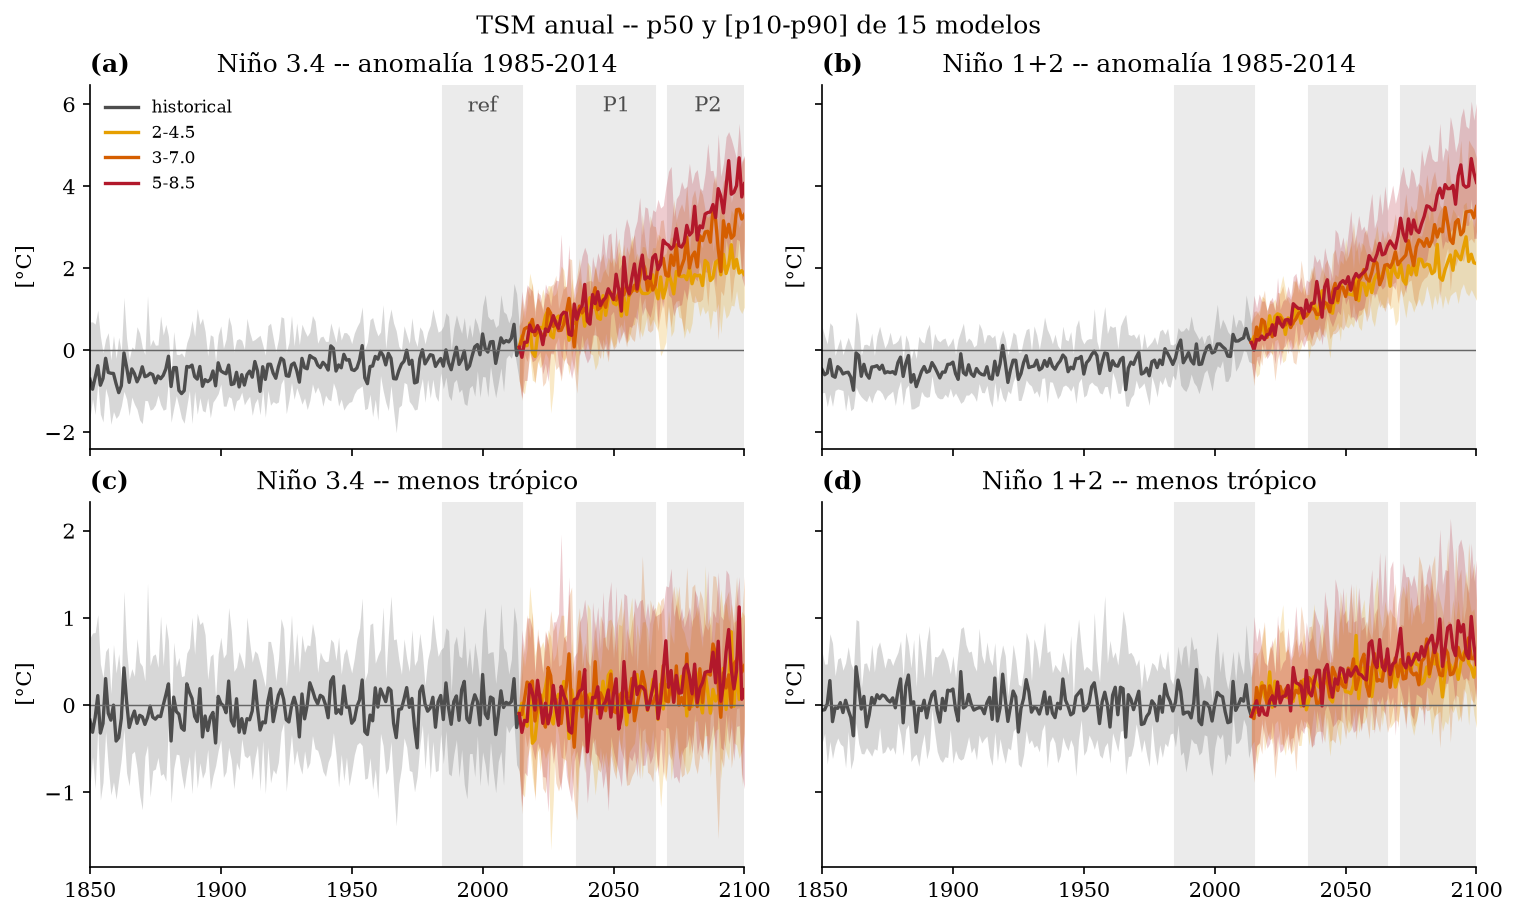
\includegraphics[width=\textwidth]{figuras/e3_01_trayectoria_tsm.png}
\caption[Trayectoria de la TSM anual 1850--2100.]{Trayectoria de la TSM anual, 1850--2100, como anomalía respecto de 1985--2014 de cada modelo. (a, b) Niño~3.4 y Niño~1+2. (c, d) La misma anomalía menos la del trópico (20°S--20°N): por encima de 0, la caja se calienta más que el trópico. Línea: mediana de los 15 modelos; sombra: percentiles 10--90. Franjas grises: ref, P1 y P2.}
\label{fig:trayectoria}
\end{figure}

Los mapas de la Figura~\ref{fig:mapas_media} muestran que el calentamiento no es uniforme. Es máximo en el Pacífico ecuatorial oriental y frente a la costa de Perú y Ecuador, donde supera los 4\,°C en P2 con SSP5-8.5, y mínimo en el Pacífico suroriental, frente a Chile. Todos los modelos coinciden en el signo en todo el dominio (no hay tramado).

\begin{figure}[htbp]
\centering
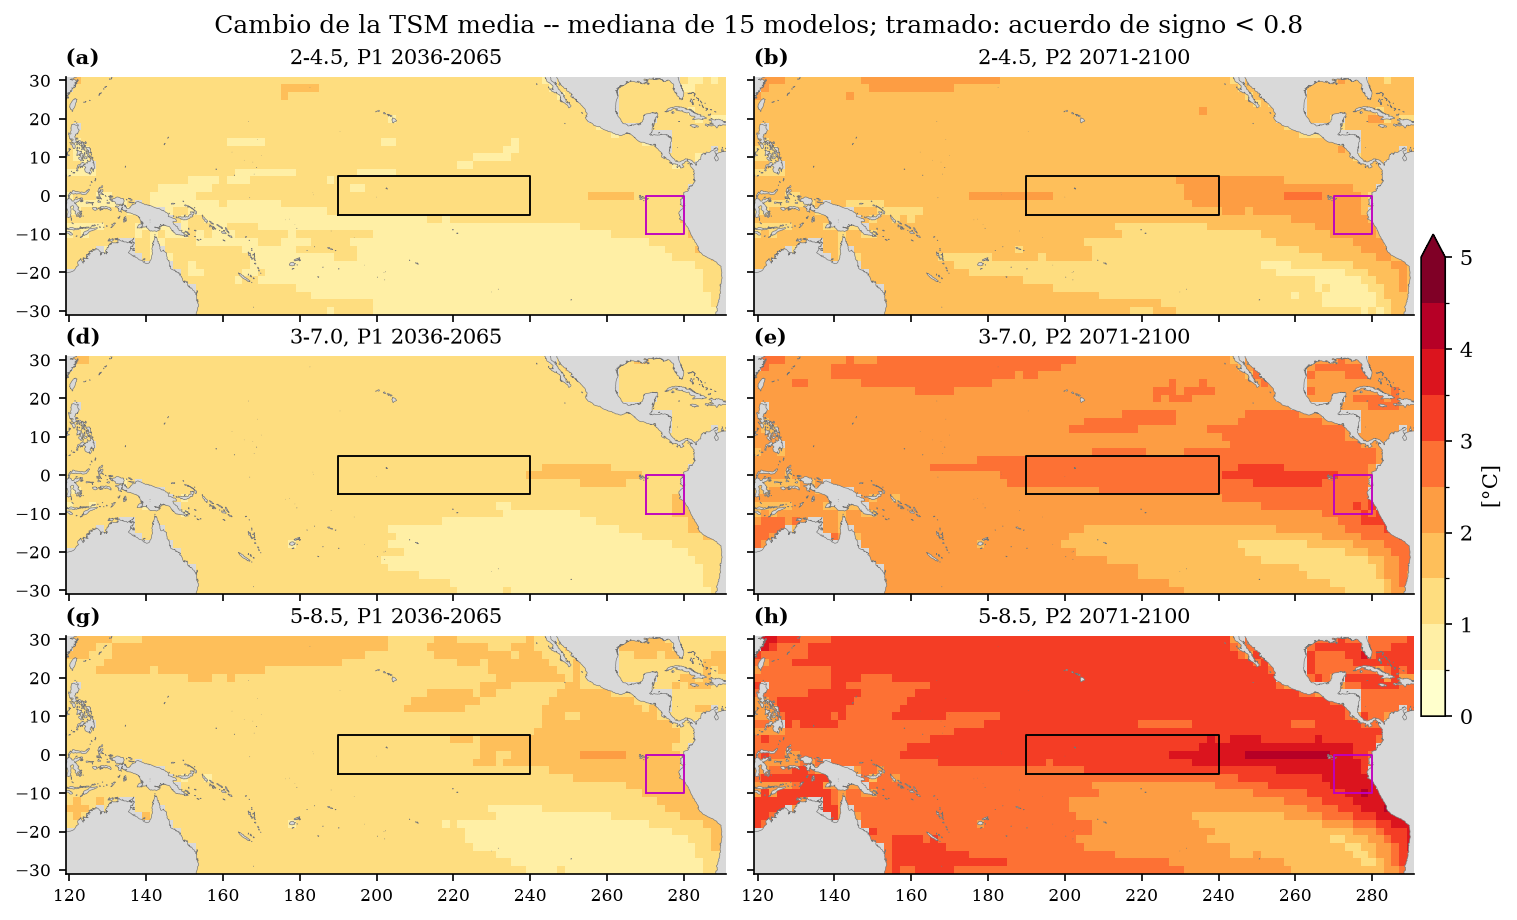
\includegraphics[width=\textwidth]{figuras/e3_02_mapas_cambio_tsm.png}
\caption[Mapas de cambio de la TSM media.]{Cambio de la TSM media (periodo futuro menos 1985--2014), mediana de los 15 modelos. Columnas: SSP2-4.5, SSP3-7.0 y SSP5-8.5; filas: P1 y P2. El tramado, ausente aquí, marcaría los puntos donde menos del 80\,\% de los modelos coincide en el signo. Recuadros: Niño~3.4 (negro) y Niño~1+2 (magenta).}
\label{fig:mapas_media}
\end{figure}

La Figura~\ref{fig:cambio_cajas} lleva estos cambios a las dos cajas, modelo por modelo. En P2, Niño~1+2 se calienta $+2.25$, $+2.79$ y $+3.64$\,°C y Niño~3.4 $+1.91$, $+2.63$ y $+3.36$\,°C con los tres escenarios; los 15 modelos coinciden en el signo y el cambio es significativo en todos los casos. La dispersión entre modelos es grande: con SSP5-8.5, Niño~1+2 va de $+2.6$ a $+5.5$\,°C. Lo que más distingue a las dos cajas es el cambio relativo (paneles c y d): Niño~1+2 se calienta entre 0.4 y 0.7\,°C más que el trópico en P2, con acuerdo de 15 de 15 modelos; en Niño~3.4 la diferencia es la mitad (0.2--0.4\,°C) y menos segura (acuerdo de 0.87 a 0.93). El cambio relativo no se somete a prueba formal: su robustez se lee en el acuerdo de signo. Su distribución en el mapa está en el Anexo (Figura~\ref{fig:mapas_rel}).

\begin{figure}[htbp]
\centering
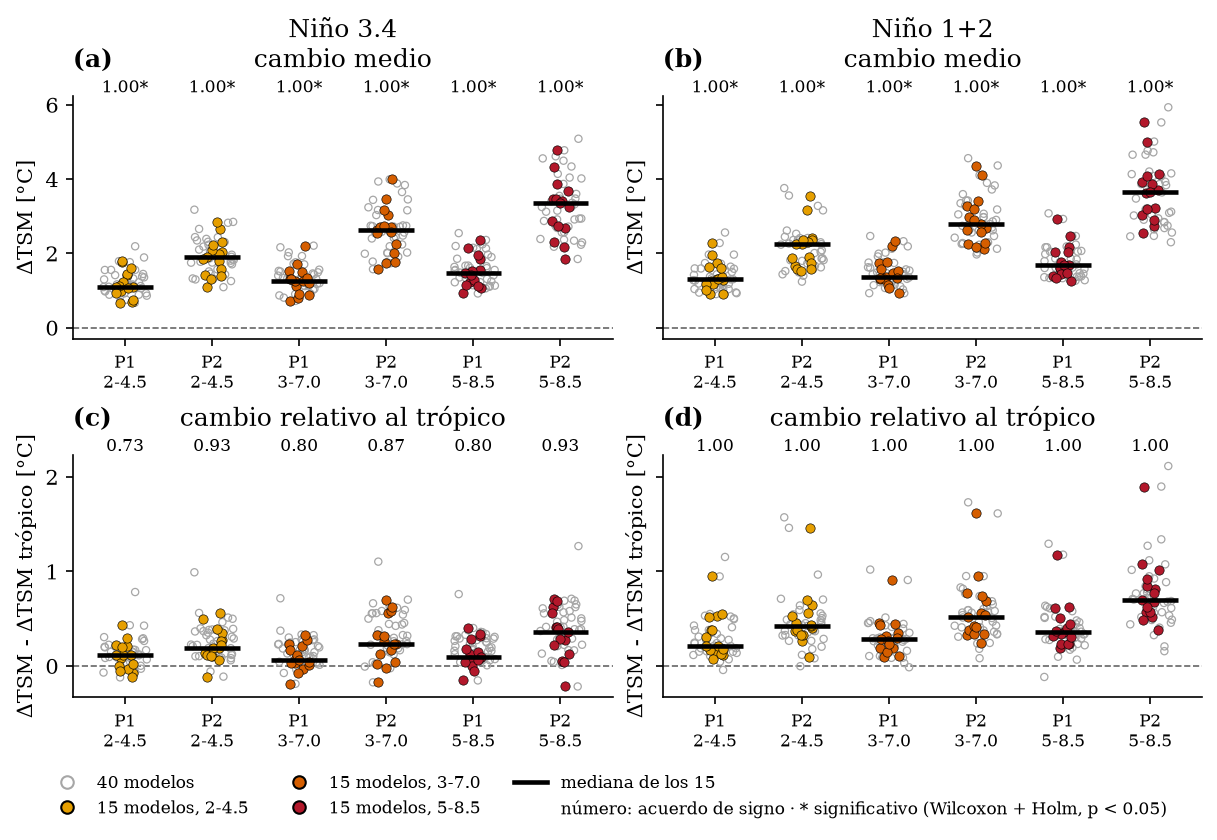
\includegraphics[width=\textwidth]{figuras/e3_03_cambio_cajas_por_modelo.png}
\caption[Cambio de la TSM media en las cajas, por modelo.]{Cambio de la TSM media en Niño~3.4 y Niño~1+2, por modelo. (a, b) Cambio total; (c, d) cambio relativo al trópico. Puntos de color: los 15 modelos; círculos grises: los 40; barra negra: mediana de los 15. Número superior: acuerdo de signo; $^{*}$: significativo con Wilcoxon y Holm (solo a y b; el cambio relativo no se prueba). Cada fila comparte la escala vertical.}
\label{fig:cambio_cajas}
\end{figure}

% ------------------------------------------------------------
\subsection{Variabilidad interanual}
\label{sec:res_var}

\textbf{Niño~3.4 tiende a una variabilidad mayor, pero los modelos no se ponen de acuerdo.} La Figura~\ref{fig:mapas_sigma} muestra el cambio de la desviación estándar de la anomalía, sin el ciclo anual ni la tendencia de cada periodo. El aumento se concentra en el Pacífico ecuatorial central, sobre Niño~3.4, con $+20$ a $+40$\,\% en P2 con SSP3-7.0 y SSP5-8.5. Casi todo el mapa está tramado: en la mayoría de los puntos menos del 80\,\% de los modelos coincide en si la variabilidad sube o baja. Frente a Perú el cambio es cercano a cero.

\begin{figure}[htbp]
\centering
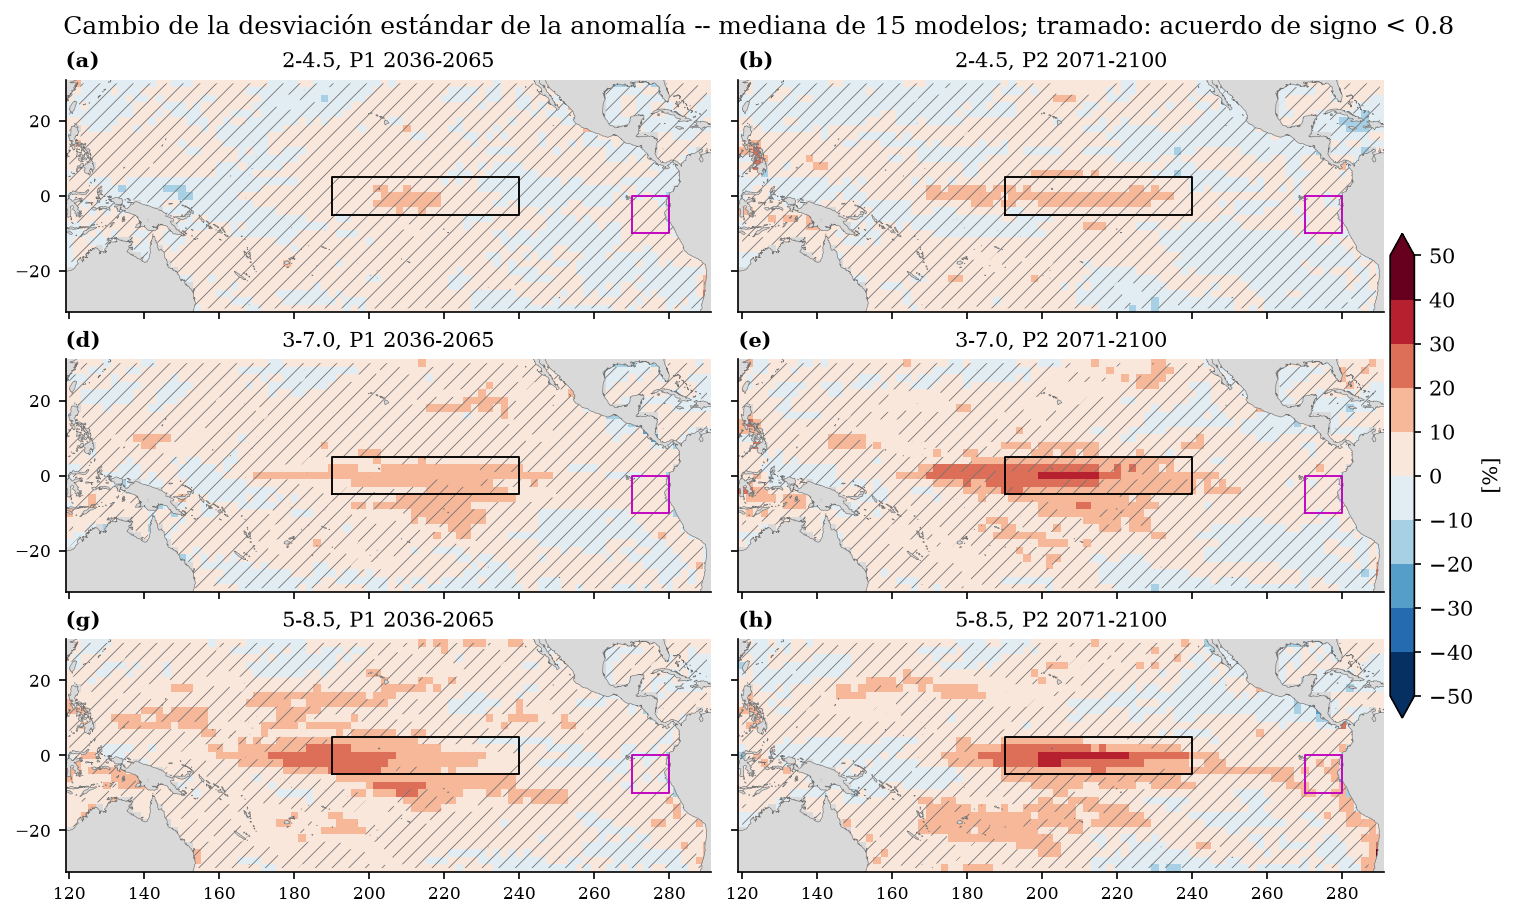
\includegraphics[width=\textwidth]{figuras/e3_04_mapas_cambio_variabilidad.png}
\caption[Mapas de cambio de la variabilidad interanual.]{Cambio porcentual de la desviación estándar de la anomalía mensual sin tendencia, $100(\sigma_P/\sigma_{\mathrm{ref}}-1)$, mediana de los 15 modelos. Tramado: acuerdo de signo menor que 0.8. Paneles como en la Figura~\ref{fig:mapas_media}.}
\label{fig:mapas_sigma}
\end{figure}

En la caja Niño~3.4 (Figura~\ref{fig:sigma}a), la mediana de $\sigma_{3m}$ sube $+11$, $+23$ y $+26$\,\% en P2. El ejemplo de la Sección~\ref{sec:multimodelo} muestra el porqué de la cautela: con SSP5-8.5, 13 de los 15 modelos proyectan aumento, pero los cambios van de $-29$ a $+105$\,\%, y tras la corrección por pruebas múltiples el resultado no es significativo. Solo P1 con SSP3-7.0 ($+15$\,\%) y con SSP5-8.5 ($+12$\,\%) pasan la prueba. En Niño~1+2 (Figura~\ref{fig:sigma}b) la mediana queda entre $-0.5$ y $+10$\,\%, con acuerdo de 8 a 12 modelos: no hay un cambio claro en la intensidad de los eventos costeros.

\begin{figure}[htbp]
\centering
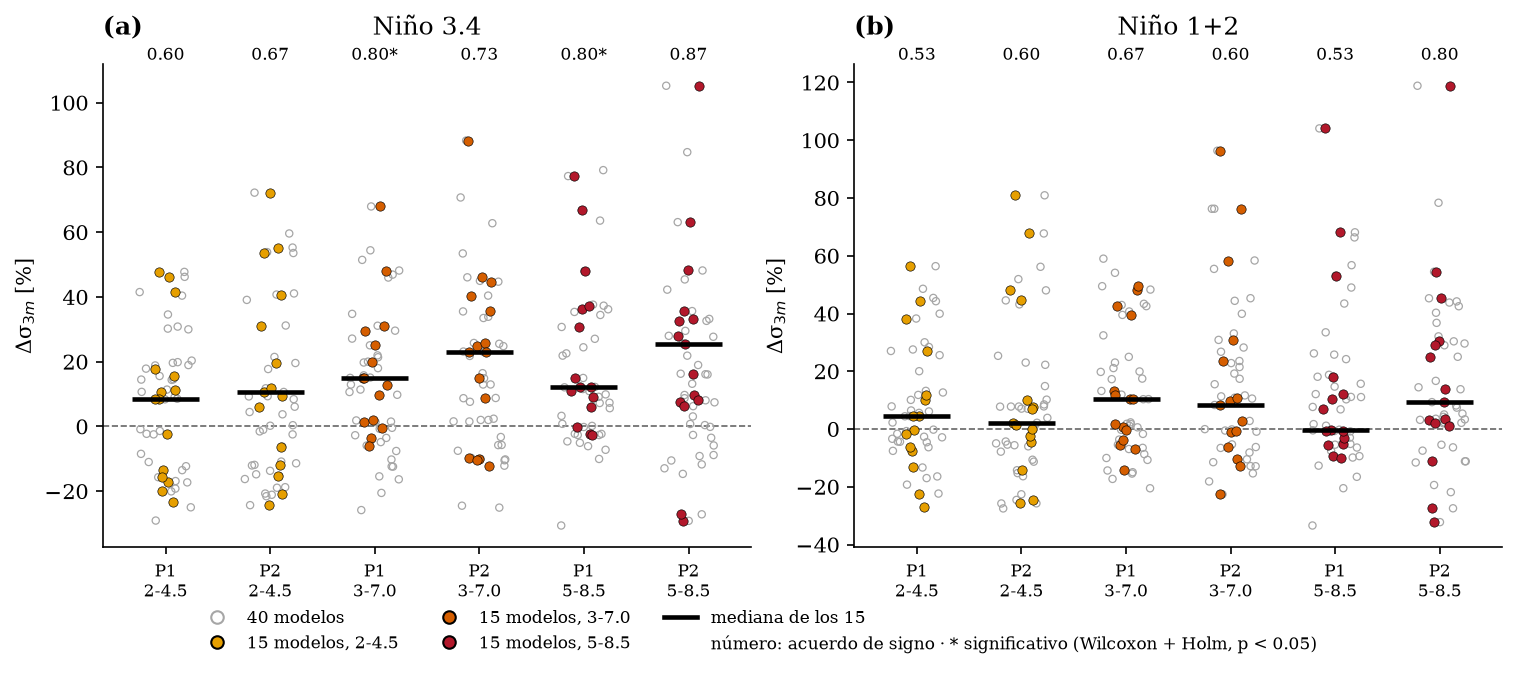
\includegraphics[width=\textwidth]{figuras/e3_05_cambio_sigma_por_modelo.png}
\caption[Cambio de la variabilidad $\sigma_{3m}$ en las cajas, por modelo.]{Cambio porcentual de $\sigma_{3m}$ (desviación estándar de la anomalía suavizada a 3 meses, la escala del ONI y del ICEN) en Niño~3.4 (a) y Niño~1+2 (b), por modelo. Formato como en la Figura~\ref{fig:cambio_cajas}.}
\label{fig:sigma}
\end{figure}

La Figura~\ref{fig:sigma_movil} muestra cómo evoluciona $\sigma_{3m}$ con ventanas de 30 años que avanzan año a año. En Niño~3.4 el aumento es gradual desde la década de 2020 y alcanza su máximo en ventanas centradas entre 2067 y 2072 ($+21$, $+29$ y $+31$\,\% con los tres escenarios). La banda entre modelos (de $-20$ a $+70$\,\%) es mucho más ancha que la variación del periodo histórico, lo que confirma que la magnitud del aumento depende fuertemente del modelo. En Niño~1+2 la mediana se mantiene casi siempre por debajo de $+10$\,\%, con un máximo de $+20$\,\% hacia 2077 con SSP5-8.5.

\begin{figure}[htbp]
\centering
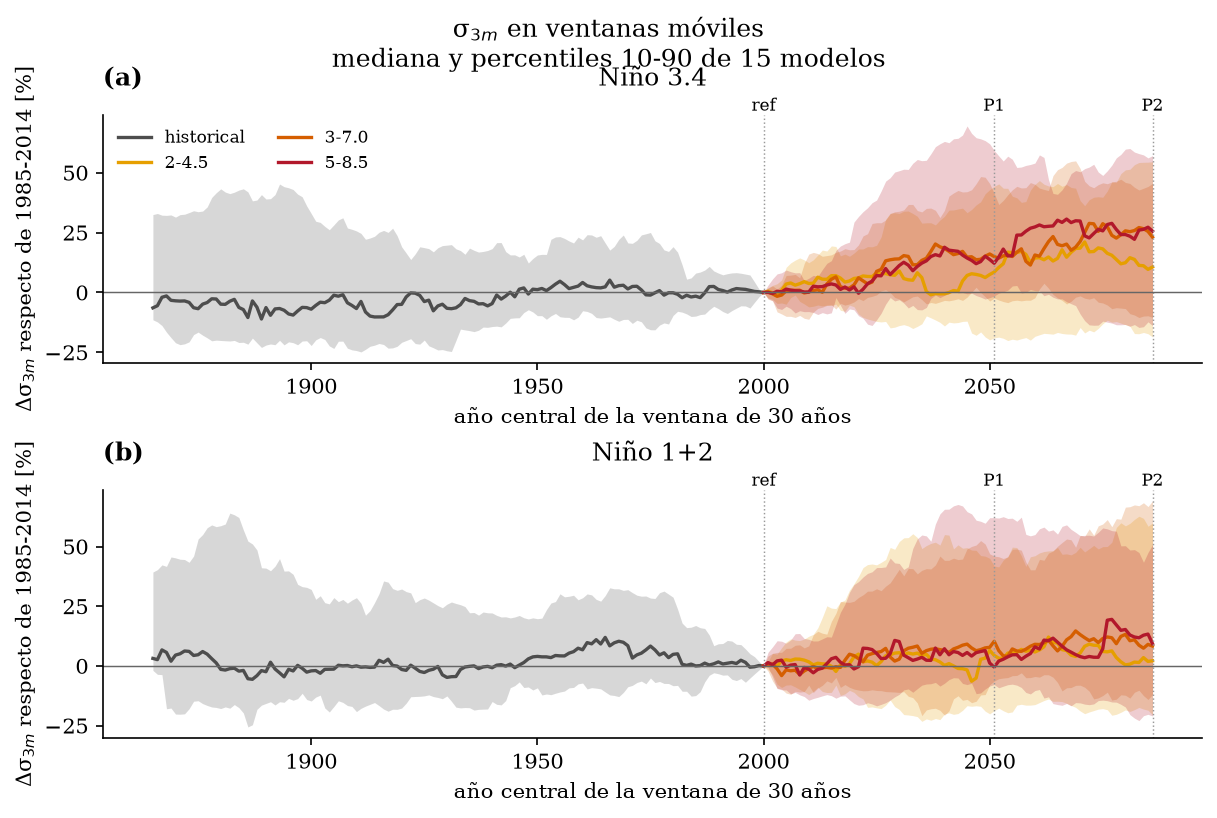
\includegraphics[width=\textwidth]{figuras/e3_06_sigma_movil.png}
\caption[Evolución de $\sigma_{3m}$ en ventanas móviles de 30 años.]{Cambio porcentual de $\sigma_{3m}$ en ventanas de 30 años que avanzan de un año en un año, respecto de la ventana centrada en 2000 (1985--2014), en Niño~3.4 (a) y Niño~1+2 (b). Eje horizontal: año central de la ventana. Línea: mediana de los 15 modelos; sombra: percentiles 10--90.}
\label{fig:sigma_movil}
\end{figure}

% ------------------------------------------------------------
\subsection{Índices ENOS: tiempo sobre el umbral}
\label{sec:res_umbral}

\textbf{La respuesta depende de con qué ``normal'' se compare.} La Figura~\ref{fig:umbral} cuenta qué fracción de los meses de cada periodo el índice está por encima del umbral de inicio de El Niño (0.5\,°C), sin exigir duración. Con los índices de base móvil (ONI, RONI, ICEN), que comparan cada mes con el clima de su época, la fracción sube poco: el ONI pasa del 31\,\% de los meses en ref al 35--41\,\% en P2, y el ICEN del 24\,\% al 29--36\,\%. Con los índices de base fija, que comparan con el clima de 1985--2014, la fracción se dispara: ONIfija pasa del 31\,\% al 88--98\,\% e ICENfija del 23\,\% al 99--100\,\%. Dicho de otro modo: a fin de siglo, la TSM de Niño~1+2 estará casi siempre por encima de lo que hoy se consideraría el inicio de un Niño costero, aunque el ENOS mismo cambie poco. Las series de los índices hasta 2100 están en el Anexo (Figuras~\ref{fig:a_indices} y \ref{fig:a_fijos}).

\begin{figure}[htbp]
\centering
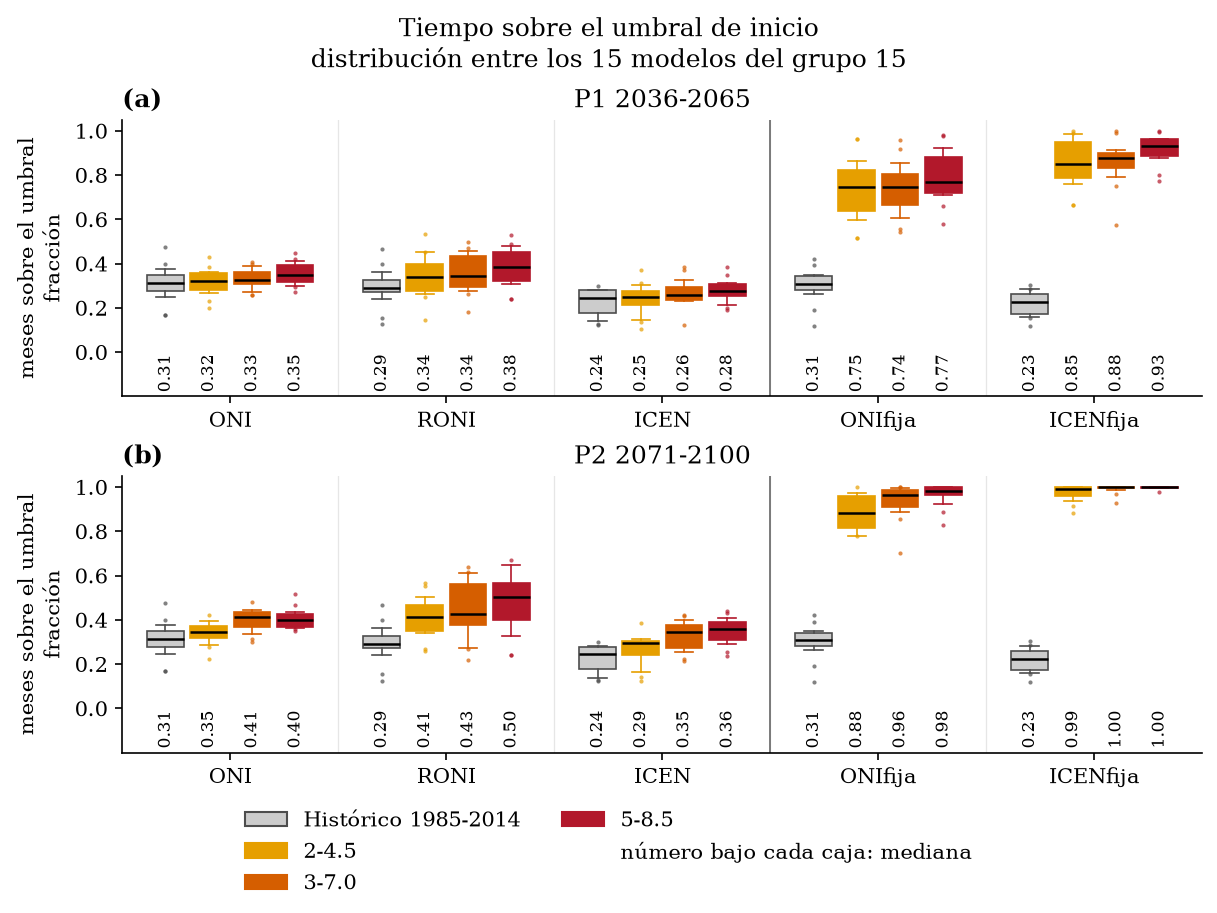
\includegraphics[width=\textwidth]{figuras/e3_07_tiempo_sobre_umbral.png}
\caption[Fracción de meses sobre el umbral de inicio de El Niño.]{Fracción de los meses de cada periodo con el índice sobre el umbral de inicio de evento, sin exigir duración, en P1 (a) y P2 (b). Izquierda de la línea vertical: índices con base móvil (ONI, RONI, ICEN); derecha: con base fija 1985--2014 (ONIfija, ICENfija). Caja: percentiles 25--75 de los 15 modelos; línea: mediana; bigotes: percentiles 10--90; número bajo cada caja: su mediana.}
\label{fig:umbral}
\end{figure}

% ------------------------------------------------------------
\subsection{Eventos cálidos}
\label{sec:res_eventos}

\textbf{Más eventos en la mediana, pero casi sin significancia.} La Figura~\ref{fig:frecuencia} compara la frecuencia de eventos de cada periodo futuro con la de ref, modelo por modelo. La mediana de la razón está por encima de 1 en casi todos los casos: en P2 los eventos del ONI aumentan 25\,\% con los tres escenarios, los del RONI entre 22 y 44\,\% y los del ICEN entre 11 y 20\,\%. En valores absolutos, el ONI pasa de 8 eventos cada 30 años en ref a 10--11 en P2, y el RONI de 9 a 11--13. Sin embargo, solo un cambio es significativo, el del RONI con SSP2-4.5 en P2 ($+30$\,\%), y el acuerdo de signo no pasa de 0.87: entre 2 y 6 de los 15 modelos no proyectan aumento. Con unos 9 eventos por periodo, duplicar la frecuencia en un solo modelo apenas sería detectable (Sección~\ref{sec:pruebas_modelo}), así que esta falta de significancia indica una señal débil frente al azar, no ausencia de cambio. Como referencia, ERSSTv5 registra en 1900--2014 el equivalente a 8 (ONI), 9 (RONI) y 11 (ICEN) eventos cada 30 años.

\begin{figure}[htbp]
\centering
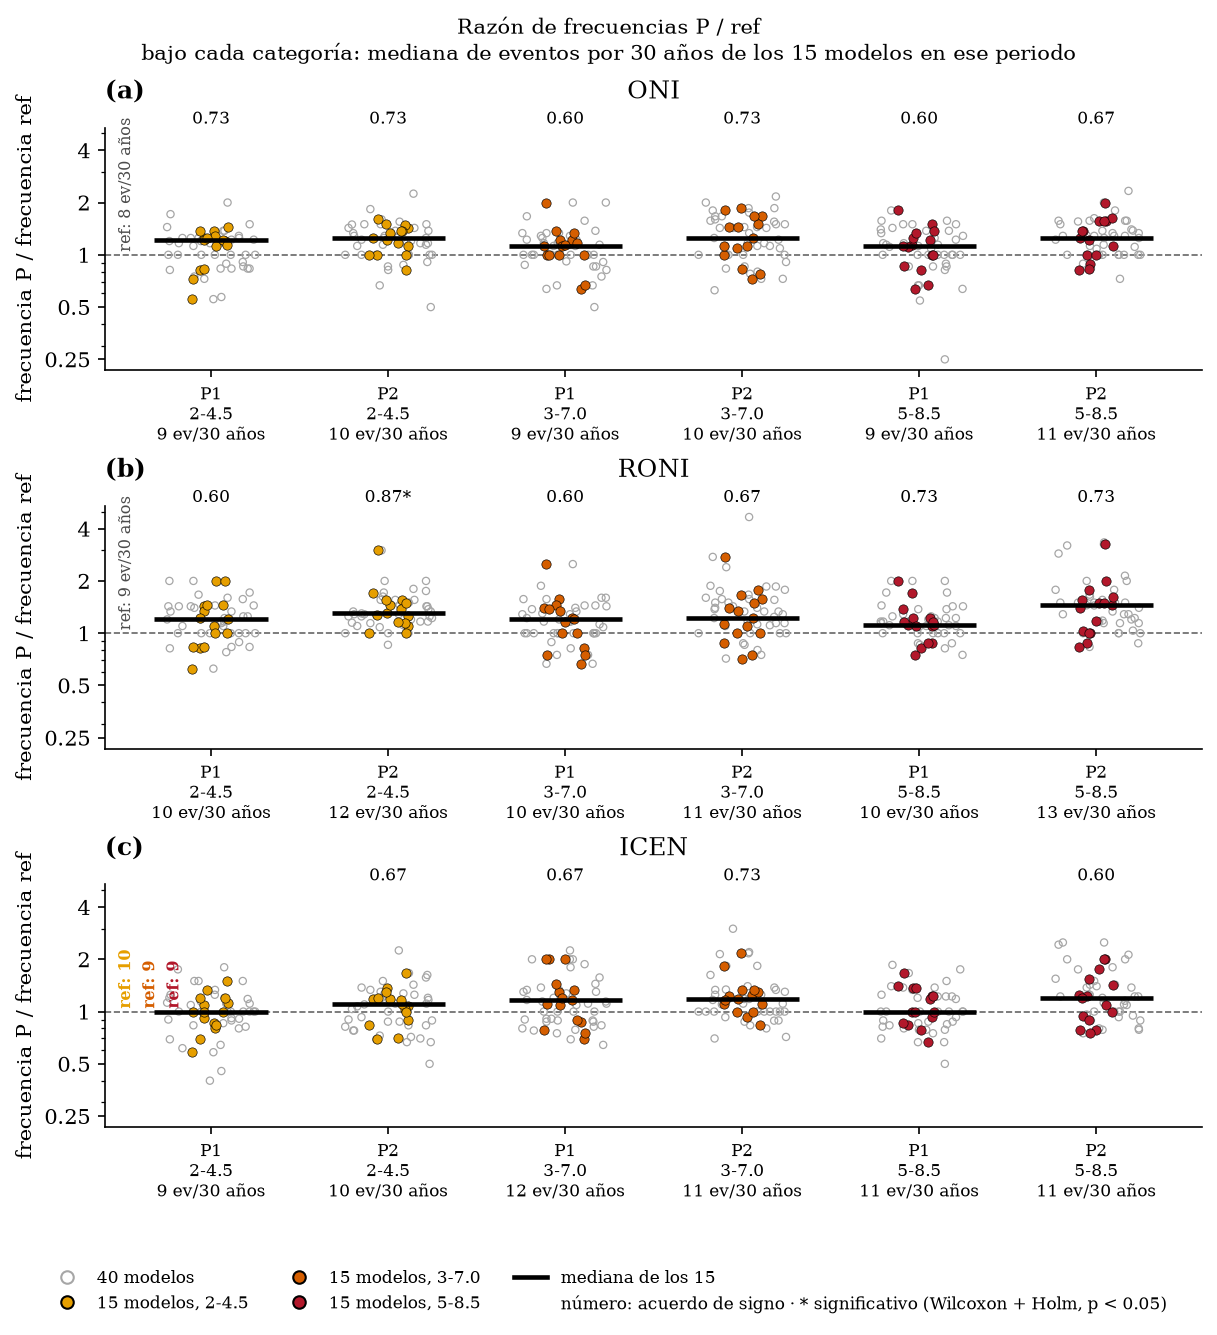
\includegraphics[width=\textwidth]{figuras/e3_08_razon_frecuencia.png}
\caption[Razón de frecuencias de eventos cálidos, P/ref.]{Razón entre la frecuencia de eventos cálidos del periodo futuro y la de 1985--2014, por modelo, para ONI (a), RONI (b) e ICEN (c); escala logarítmica, en la que duplicar y reducir a la mitad quedan a la misma distancia de 1. Bajo cada columna: mediana de los 15 modelos en eventos por 30 años (el largo de cada periodo); junto a la línea 1: la mediana en ref (en ICEN difiere entre escenarios y se da con el color de cada uno). Formato como en la Figura~\ref{fig:cambio_cajas}.}
\label{fig:frecuencia}
\end{figure}

\textbf{Los eventos tienden a ser más intensos.} La Figura~\ref{fig:caracteristicas} compara otras características de los eventos entre periodos. El cambio más claro es el de los \textbf{eventos extremos}: el número de eventos fuertes o más intensos, según la escala oficial, sube de 3 a 5--7 por cada 30 años en el ONI y de 3 a 5--9 en el RONI, y el aumento es significativo con SSP3-7.0 y SSP5-8.5 en ambos periodos (en el RONI, también con SSP2-4.5 en P2). En el ICEN, que parte de casi ningún evento fuerte en ref, el aumento (a 1--2) no es significativo. Además, los eventos del ICEN duran más (de 8.0 a 10.1 y 11.0 meses en P1 y P2 con SSP5-8.5, y a 9.2 con SSP3-7.0 en P2, significativo), y el pico medio de los eventos del RONI sube con SSP3-7.0 y SSP5-8.5 (de 1.38 a 1.7--2.0\,°C, significativo). Los eventos que superan dos veces la $\sigma$ de la referencia (extremos relativos, sin prueba formal) pasan, con SSP5-8.5, de 1 a 5 por cada 30 años en ONI y RONI. Todo esto es coherente con el aumento de variabilidad de Niño~3.4.

\begin{figure}[htbp]
\centering
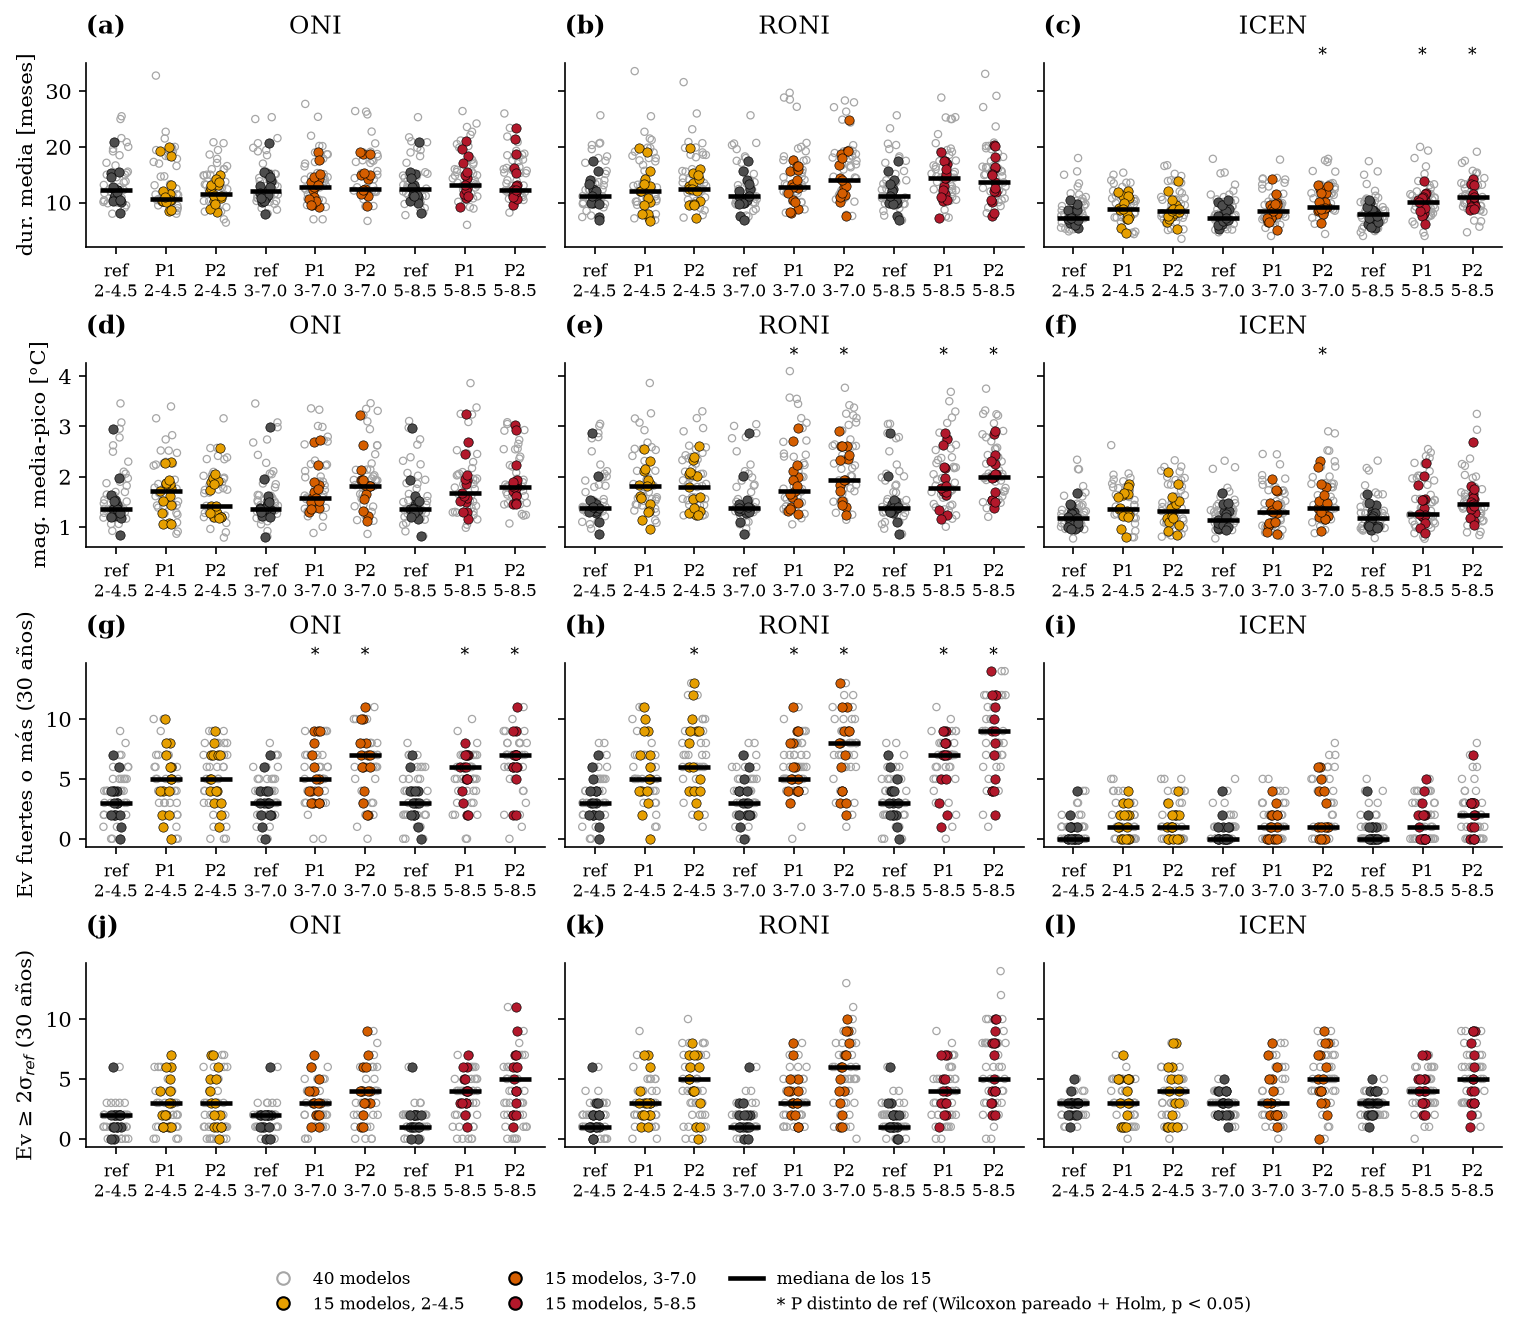
\includegraphics[width=\textwidth]{figuras/e3_09_duracion_magnitud.png}
\caption[Duración, magnitud y número de eventos intensos.]{Características de los eventos cálidos por periodo, para ONI, RONI e ICEN (columnas). Filas: duración media (meses), magnitud media del pico (°C), número de eventos fuertes o más intensos según la escala oficial y número de eventos con pico $\geq 2\sigma_{\mathrm{ref}}$, ambos por periodo de 30 años. Puntos gris oscuro: ref; $^{*}$: el periodo difiere de ref (Wilcoxon pareado y Holm).}
\label{fig:caracteristicas}
\end{figure}

\clearpage
% ------------------------------------------------------------
\subsection{Síntesis}
\label{sec:res_sintesis}

El Cuadro~\ref{tab:sintesis} reúne la mediana del cambio de las variables principales en los seis casos (tres escenarios por dos periodos), en el orden de los puntos del TdR. Se lee por bloques. \textbf{Estado medio:} el calentamiento es robusto y significativo en todos los casos y crece con el escenario; el calentamiento relativo de Niño~1+2 es robusto en todos los casos, aunque no se somete a prueba. \textbf{Variabilidad:} medianas positivas, pero rara vez robustas y solo significativas en P1 con SSP3-7.0 y SSP5-8.5 en Niño~3.4. \textbf{Eventos:} la frecuencia con base móvil sube en la mediana, pero solo es significativa en un caso; los eventos fuertes o más intensos del ONI y del RONI, en cambio, aumentan de forma significativa con SSP3-7.0 y SSP5-8.5. La frecuencia con base fija \emph{baja} en P2, no porque haya menos calor, sino porque el índice queda sobre el umbral casi todo el tiempo y los eventos se funden en uno o dos episodios muy largos (Sección~\ref{sec:eventos}); para esos índices la medida correcta es el tiempo sobre el umbral (Figura~\ref{fig:umbral}). Estas medianas casi no cambian al usar 40, 11 o 7 modelos en lugar de 15 (Anexo, Figura~\ref{fig:a_sensibilidad}).

\begin{table}[htbp]
\caption[Síntesis del cambio proyectado (15 modelos).]{Síntesis del cambio proyectado: mediana de los 15 modelos. En negrita, cambios robustos (acuerdo de signo $\geq 0.8$); $^{*}$: significativo con Wilcoxon y corrección de Holm ($p<0.05$). El cambio relativo no se somete a prueba (Sección~\ref{sec:multimodelo}). Las razones de frecuencia se comparan con 1 (sin cambio); los eventos fuertes o más intensos (número por periodo de 30 años, sin negrita porque no es un cambio respecto de un valor neutro), con su número en ref; el resto, con 0.}
\label{tab:sintesis}
\centering
\footnotesize
\setlength{\tabcolsep}{4pt}
\begin{tabular}{@{}lrrrrrr@{}}
\toprule
 & \multicolumn{2}{c}{\textbf{SSP2-4.5}} & \multicolumn{2}{c}{\textbf{SSP3-7.0}} & \multicolumn{2}{c}{\textbf{SSP5-8.5}} \\
\cmidrule(lr){2-3}\cmidrule(lr){4-5}\cmidrule(l){6-7}
\textbf{Variable} & \textbf{P1} & \textbf{P2} & \textbf{P1} & \textbf{P2} & \textbf{P1} & \textbf{P2} \\
\midrule
$\Delta$TSM Niño~3.4 [°C] & \textbf{+1.10}$^{*}$ & \textbf{+1.91}$^{*}$ & \textbf{+1.25}$^{*}$ & \textbf{+2.63}$^{*}$ & \textbf{+1.48}$^{*}$ & \textbf{+3.36}$^{*}$ \\
$\Delta$TSM Niño~1+2 [°C] & \textbf{+1.30}$^{*}$ & \textbf{+2.25}$^{*}$ & \textbf{+1.36}$^{*}$ & \textbf{+2.79}$^{*}$ & \textbf{+1.69}$^{*}$ & \textbf{+3.64}$^{*}$ \\
$\Delta$TSM rel. Niño~3.4 [°C] & +0.11 & \textbf{+0.19} & \textbf{+0.07} & \textbf{+0.23} & \textbf{+0.09} & \textbf{+0.36} \\
$\Delta$TSM rel. Niño~1+2 [°C] & \textbf{+0.22} & \textbf{+0.42} & \textbf{+0.29} & \textbf{+0.51} & \textbf{+0.36} & \textbf{+0.70} \\
\midrule
$\Delta\sigma_{3m}$ Niño~3.4 [\%] & +9 & +11 & \textbf{+15}$^{*}$ & +23 & \textbf{+12}$^{*}$ & \textbf{+26} \\
$\Delta\sigma_{3m}$ Niño~1+2 [\%] & +4 & +2 & +10 & +8 & 0 & \textbf{+9} \\
\midrule
Frecuencia P/ref, ONI & 1.22 & 1.25 & 1.12 & 1.25 & 1.12 & 1.25 \\
Frecuencia P/ref, RONI & 1.20 & \textbf{1.30}$^{*}$ & 1.20 & 1.22 & 1.11 & 1.44 \\
Frecuencia P/ref, ICEN & 1.00 & 1.11 & 1.17 & 1.18 & 1.00 & 1.20 \\
Frecuencia P/ref, ONIfija & 1.22 & 1.00 & 1.00 & \textbf{0.56}$^{*}$ & 0.89 & \textbf{0.25}$^{*}$ \\
Frecuencia P/ref, ICENfija & 0.92 & \textbf{0.29}$^{*}$ & 0.89 & \textbf{0.11}$^{*}$ & 0.62 & \textbf{0.11}$^{*}$ \\
\midrule
Eventos fuertes+, ONI (ref: 3) & 5 & 5 & 5$^{*}$ & 7$^{*}$ & 6$^{*}$ & 7$^{*}$ \\
Eventos fuertes+, RONI (ref: 3) & 5 & 6$^{*}$ & 5$^{*}$ & 8$^{*}$ & 7$^{*}$ & 9$^{*}$ \\
Eventos fuertes+, ICEN (ref: 0) & 1 & 1 & 1 & 1 & 1 & 2 \\
\bottomrule
\end{tabular}
\end{table}

% ============================================================
\section{Limitaciones}
\label{sec:limitaciones}
% ============================================================

\begin{itemize}[nosep]
\item \textbf{Un miembro por modelo.} Cada modelo aporta una sola realización. En 30 años, la variabilidad interna de esa corrida puede producir o borrar diferencias de frecuencia y de $\sigma$ sin que cambie la física del modelo. Separar ese efecto es parte del Entregable~4.
\item \textbf{Pocos eventos por periodo.} Con unos 9 eventos por periodo de 30 años, las pruebas por modelo detectan solo cambios muy grandes (Sección~\ref{sec:pruebas_modelo}), y la conclusión sobre eventos descansa en la mediana del conjunto, que en la frecuencia rara vez alcanza significancia. Salvo el aumento de eventos fuertes, los cambios de eventos deben leerse como tendencias probables, no como hechos establecidos.
\item \textbf{Modelos no independientes.} Modelos de un mismo centro comparten componentes (por ejemplo, CNRM-CM6-1, CNRM-CM6-1-HR y CNRM-ESM2-1), por lo que la prueba de Wilcoxon es optimista y el acuerdo de signo puede sobrestimar la robustez.
\item \textbf{Sesgos que no se cancelan.} Comparar cada modelo consigo mismo cancela su error fijo, pero no los errores que dependen del estado del océano. El Entregable~2 mostró un ciclo anual demasiado plano y una variabilidad débil en Niño~1+2; esos errores pueden afectar también al cambio proyectado en esa caja.
\item \textbf{Asimetría de los Niños costeros.} Los modelos no reproducen la asimetría del ICEN observado (Entregable~2), es decir, los Niños costeros extraordinarios como 1982--1983 y 1997--1998. Las proyecciones de eventos intensos en Niño~1+2 heredan esa limitación (Anexo, Figura~\ref{fig:a_asimetria}).
\end{itemize}

% ============================================================
\section{Conclusiones}
\label{sec:conclusiones}
% ============================================================

En cumplimiento de la actividad~(c) del TdR, con los 15 modelos seleccionados en el Entregable~2:

\begin{enumerate}[label=(\roman*)]
\item \textbf{Estado medio.} El calentamiento es el resultado más seguro: todos los modelos lo proyectan. En 2071--2100, Niño~1+2 sube $+2.3$, $+2.8$ y $+3.6$\,°C con SSP2-4.5, SSP3-7.0 y SSP5-8.5, y 0.4--0.7\,°C más que el trópico. Hasta mediados de siglo los escenarios casi no se distinguen.
\item \textbf{Variabilidad.} La de Niño~3.4 tiende a aumentar ($+11$ a $+26$\,\% en P2), sin acuerdo suficiente entre modelos; en Niño~1+2 no cambia de forma clara.
\item \textbf{Eventos extremos.} Los eventos fuertes o más intensos del ONI y del RONI pasan de 3 a 5--9 por cada 30 años con SSP3-7.0 y SSP5-8.5, de forma significativa. La frecuencia total sube 11--44\,\% en la mediana, pero casi nunca de forma significativa.
\item \textbf{Umbrales actuales.} Respecto del clima de hoy, Niño~1+2 estará sobre el umbral de El Niño casi todo el tiempo a fin de siglo, por el calentamiento de fondo y no por un ENOS más activo.
\end{enumerate}

% ============================================================
\section{Recomendaciones}
\label{sec:recomendaciones}
% ============================================================

\begin{itemize}
\item Comunicar por separado el calentamiento de fondo, que es seguro, y el cambio del ENOS, que es probable pero incierto.
\item En el monitoreo futuro, mantener índices de base móvil o relativos (ICEN, RONI), para que los umbrales detecten eventos y no solo el calentamiento.
\item En el Entregable~4, cuantificar cuánto de la dispersión entre modelos en la variabilidad y los eventos se debe a la variabilidad interna.
\end{itemize}

% ============================================================
\bibliographystyle{plainnat}
\bibliography{references}

% ============================================================
\clearpage
\appendix
\renewcommand{\thefigure}{A\arabic{figure}}
\setcounter{figure}{0}
\section{Análisis complementarios}
\label{sec:anexo}
% ============================================================

Este anexo reúne análisis que ayudan a interpretar los resultados, pero que no forman parte de lo que pide la actividad~(c) del TdR (estado medio, variabilidad y ocurrencia de eventos extremos con ONI e ICEN). Cada uno incluye su método y su resultado.

\subsection{Patrón del calentamiento relativo al trópico}
\label{sec:a_patron}

La Figura~\ref{fig:mapas_rel} resta a cada punto el calentamiento medio del trópico del mismo modelo, para ver el \emph{patrón}. Aparece una franja de calentamiento extra a lo largo del ecuador oriental que llega a la costa de Perú, y una zona que se calienta menos que el trópico al sur, entre 10°S y 30°S. Ambas son robustas (sin tramado) y se intensifican con el escenario. Es el patrón ``tipo El Niño'' descrito por \citet{xie2010}: no un Niño más frecuente, sino un fondo más cálido justo donde se desarrollan los Niños costeros.

\begin{figure}[htbp]
\centering
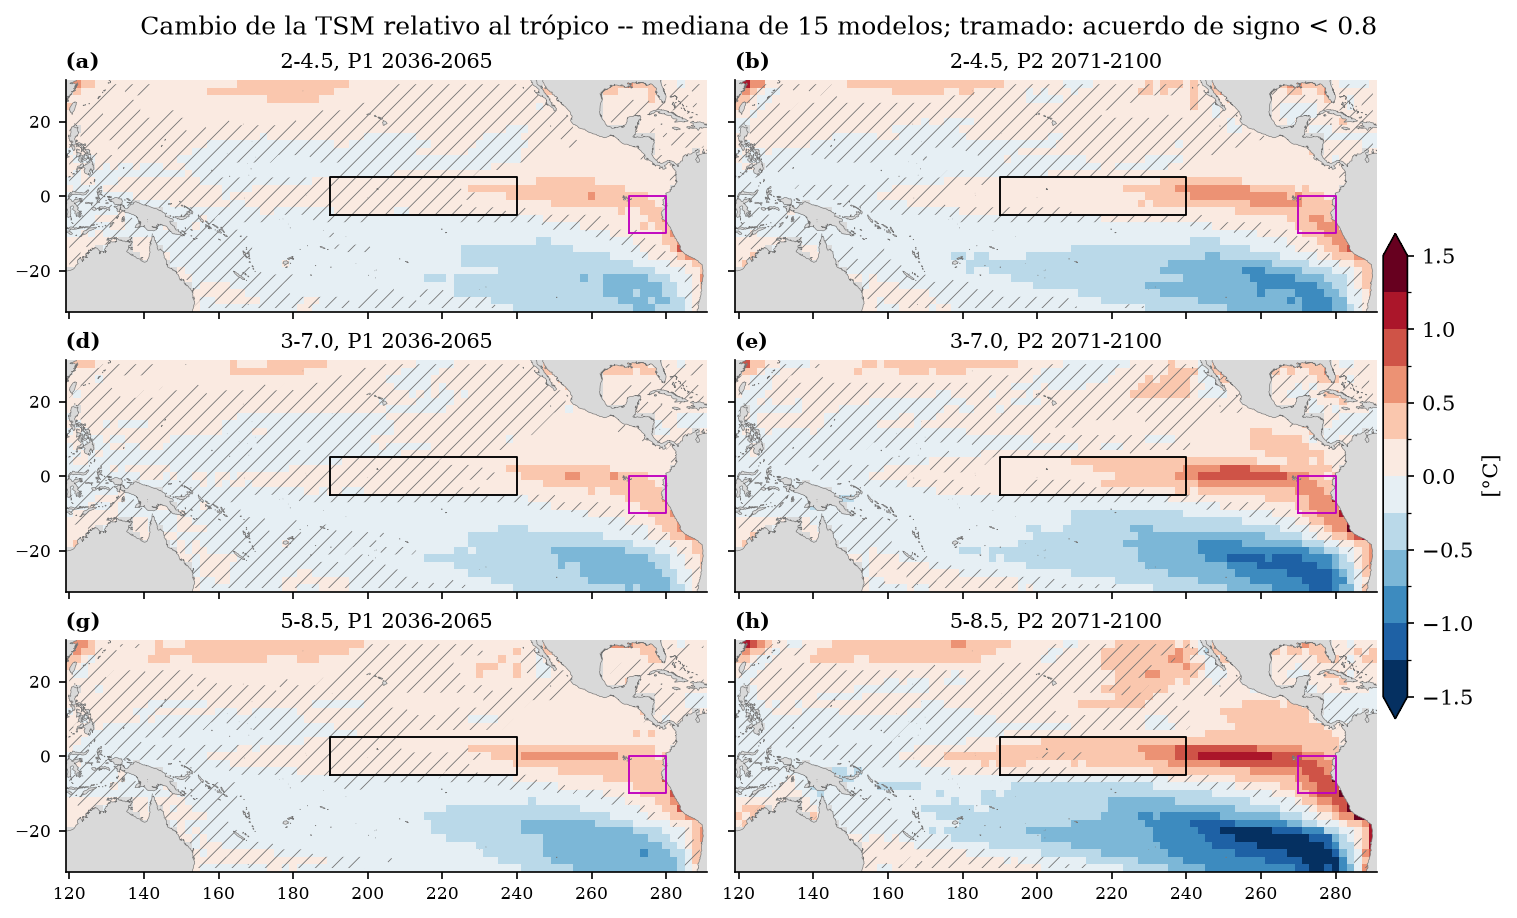
\includegraphics[width=\textwidth]{figuras/e3_A01_mapas_cambio_relativo.png}
\caption[Mapas del cambio de la TSM relativo al trópico.]{Cambio de la TSM relativo al trópico: cambio de cada punto menos el cambio medio de 20°S--20°N del mismo modelo, mediana de los 15 modelos. Rojo: se calienta más que el trópico; azul: menos. Tramado: acuerdo de signo menor que 0.8. Paneles como en la Figura~\ref{fig:mapas_media}.}
\label{fig:mapas_rel}
\end{figure}

\subsection{Ciclo anual}
\label{sec:ciclo}

\textbf{Dato:} la TSM mensual de cada periodo. \textbf{Qué se hace:} se promedian todos los eneros, todos los febreros, etc., de los 30 años; esos 12 valores son el \textbf{ciclo anual} o climatología. Su \textbf{amplitud} es la diferencia entre el mes más cálido y el más frío. En M03, la amplitud de Niño~3.4 crece 1.0\,°C en P2.

\textbf{Por qué:} en Niño~1+2 el ciclo anual (verano cálido en marzo, invierno frío en septiembre) es tan grande como un Niño fuerte. Un cambio en su amplitud cambia qué tan cálidos son los veranos ``normales'' frente a la costa, aunque no cambie el ENOS. También se registra en qué mes ocurren el máximo y el mínimo, para ver si las estaciones se adelantan o se atrasan.

\noindent\textbf{Definición formal.} Con $X(a,m)$ la TSM del año $a$ y el mes $m$, y $N_a = 30$ años,
\begin{equation}
\label{eq:amplitud}
C_m = \frac{1}{N_a}\sum_{a} X(a,m), \qquad \mathcal{A} = \max_m C_m - \min_m C_m, \qquad \Delta\mathcal{A} = \mathcal{A}_P - \mathcal{A}_{\mathrm{ref}} ,
\end{equation}
y además $\arg\max_m C_m$ y $\arg\min_m C_m$.

\textbf{Niño~1+2 se calienta más en invierno que en verano, y su ciclo anual se aplana.} La Figura~\ref{fig:ciclo} compara, mes a mes, la TSM de referencia (gris) con la de cada escenario; el número bajo cada caja es el calentamiento de ese mes. Un ejemplo: en Niño~1+2, marzo pasa de 28.1\,°C a 31.6\,°C en P2 con SSP5-8.5 ($+3.3$\,°C), mientras que agosto pasa de 22.8 a 27.0\,°C ($+3.8$\,°C). Como el mes frío sube más que el cálido, la diferencia entre ambos se reduce. Lo mismo ocurre, en menor grado, con los otros dos escenarios: con SSP2-4.5 el calentamiento es de $+2.0$\,°C en verano y $+2.4$\,°C en invierno. En Niño~3.4 sucede lo contrario: el máximo de abril--mayo sube algo más que el mínimo de septiembre--octubre ($+3.3$ a $+3.5$ frente a $+3.0$\,°C con SSP5-8.5), y el ciclo se amplifica.

\begin{figure}[htbp]
\centering
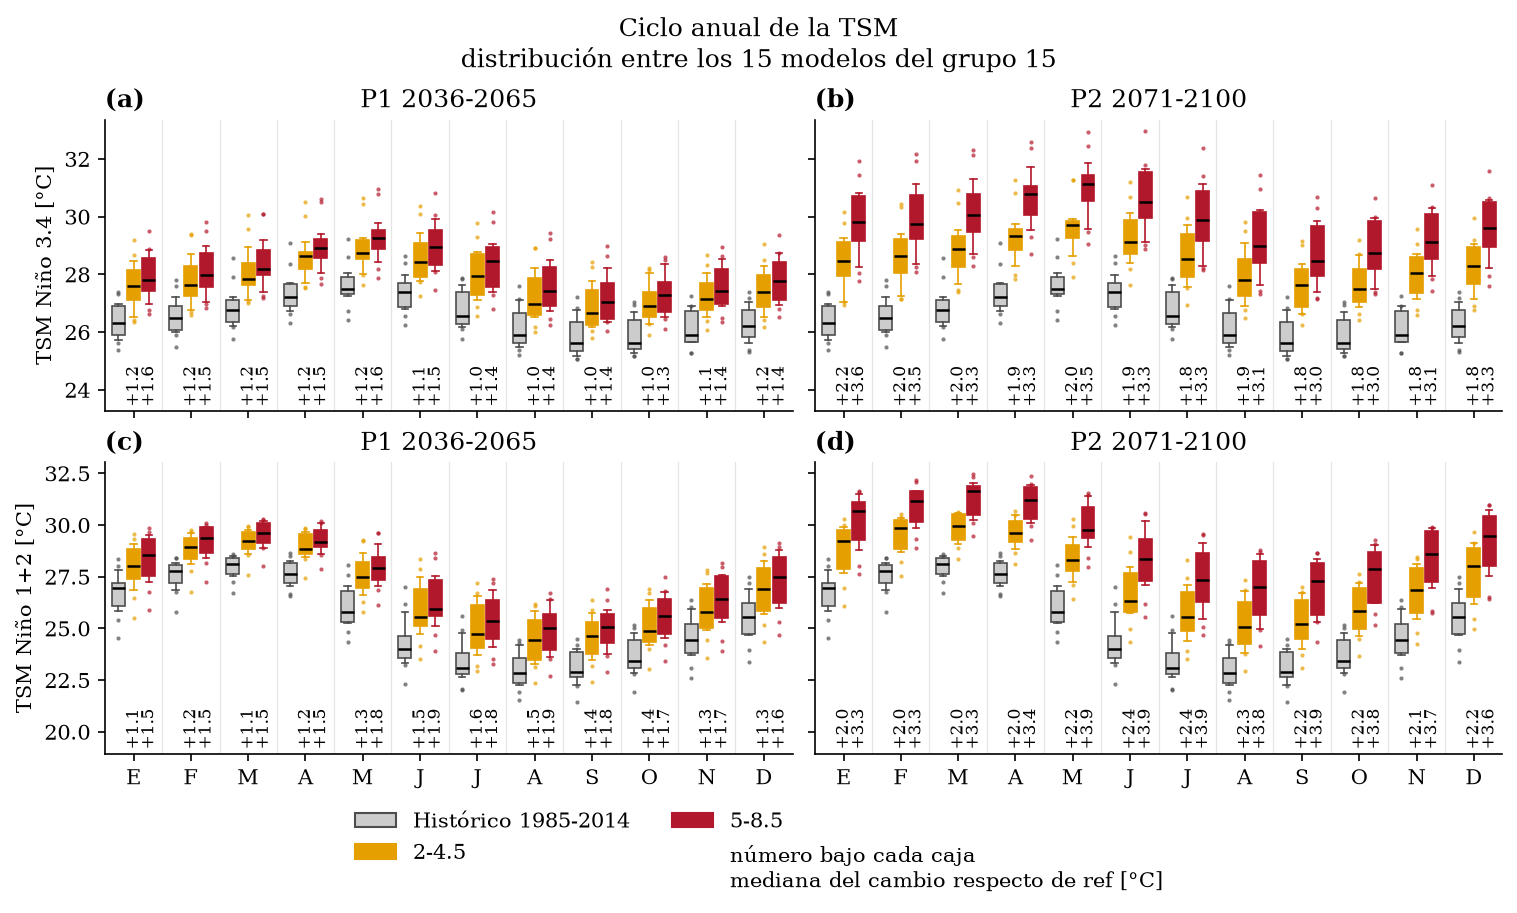
\includegraphics[width=\textwidth]{figuras/e3_A02_ciclo_anual.png}
\caption[Ciclo anual de la TSM por periodo y escenario.]{Ciclo anual de la TSM: en cada mes, distribución de la climatología de los 15 modelos (caja: percentiles 25--75; línea: mediana; bigotes: percentiles 10--90). Gris: referencia 1985--2014; color: escenarios. Filas: Niño~3.4 y Niño~1+2; columnas: P1 y P2. Número bajo cada caja: mediana del cambio de ese mes respecto de la referencia [°C], calculado modelo por modelo.}
\label{fig:ciclo}
\end{figure}

La Figura~\ref{fig:amplitud} resume ese efecto con la amplitud (mes más cálido menos mes más frío) de cada modelo. En Niño~1+2 la amplitud baja en P2 entre 0.36 y 0.49\,°C, con acuerdo de 13 o 14 de 15 modelos; en Niño~3.4 sube entre 0.13 y 0.40\,°C, también con acuerdo alto. Son cambios pequeños frente a la amplitud actual de Niño~1+2 (unos 5\,°C), pero van en el mismo sentido que el error de los modelos señalado en el Entregable~2, que ya simulan un ciclo anual demasiado plano en esa caja.

\begin{figure}[htbp]
\centering
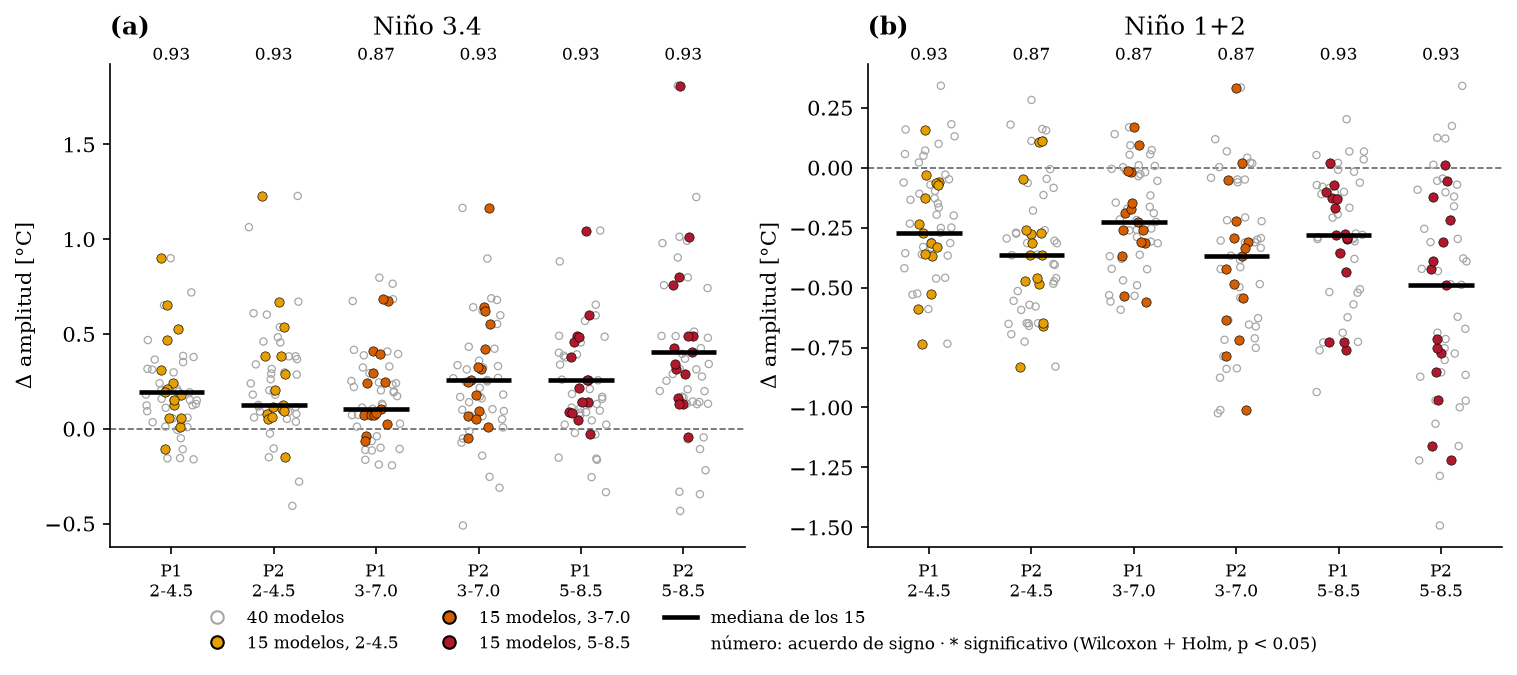
\includegraphics[width=\textwidth]{figuras/e3_A03_cambio_amplitud_por_modelo.png}
\caption[Cambio de la amplitud del ciclo anual, por modelo.]{Cambio de la amplitud del ciclo anual (máximo menos mínimo de la climatología mensual) en Niño~3.4 (a) y Niño~1+2 (b), por modelo. Formato como en la Figura~\ref{fig:cambio_cajas}; esta variable no se somete a prueba, por lo que no lleva asterisco.}
\label{fig:amplitud}
\end{figure}

\subsection{Variabilidad por estación}

La Figura~\ref{fig:a_estacional} muestra en qué época del año cambia la variabilidad ($\sigma_{3m}$ de cada trimestre, Sección~\ref{sec:variabilidad}). En Niño~3.4, el aumento de $\sigma_{3m}$ se concentra entre agosto y diciembre, cuando los Niños crecen hacia su pico; con SSP3-7.0 la mediana de noviembre--diciembre pasa de 1.0 a 1.4\,°C en P2. En Niño~1+2 las curvas se superponen y la dispersión entre modelos domina.

\begin{figure}[htbp]
\centering
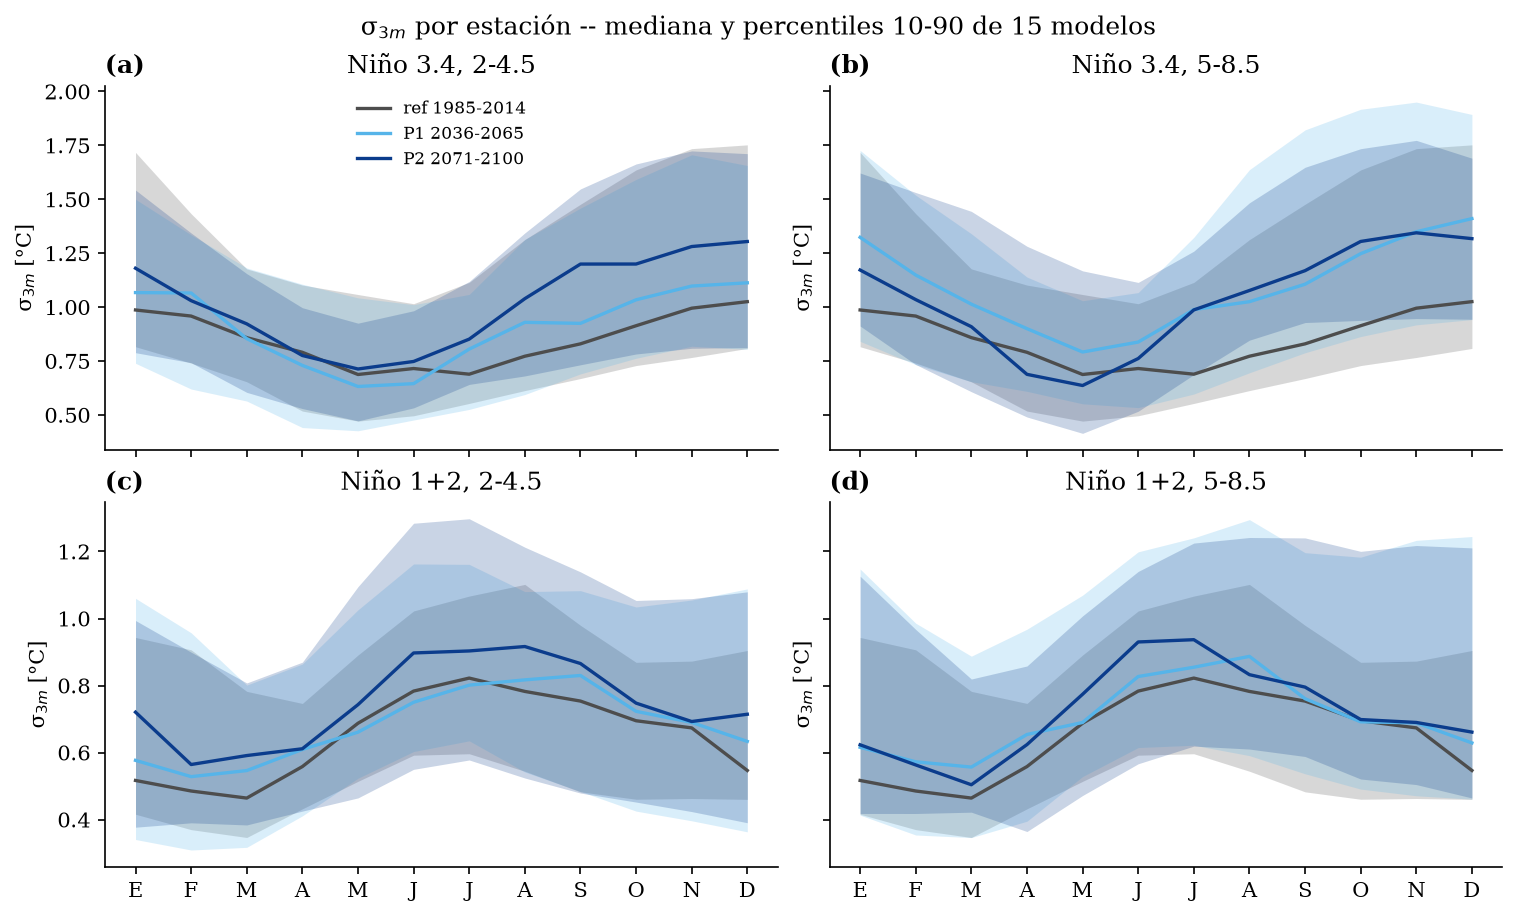
\includegraphics[width=\textwidth]{figuras/e3_A04_sigma_estacional.png}
\caption[$\sigma_{3m}$ por estación.]{$\sigma_{3m}$ por estación: desviación estándar de la anomalía suavizada en el trimestre centrado en cada mes (``E'' = diciembre--febrero), en Niño~3.4 (arriba) y Niño~1+2 (abajo), por escenario. Gris: ref; celeste: P1; azul oscuro: P2. Línea: mediana de los 15 modelos; sombra: percentiles 10--90.}
\label{fig:a_estacional}
\end{figure}

\subsection{Asimetría y curtosis}

\textbf{Dato:} la anomalía mensual sin tendencia. \textbf{Qué miden:} la \textbf{asimetría} indica si las anomalías cálidas llegan más lejos que las frías. Es positiva cuando hay pocos Niños muy intensos y muchas Niñas moderadas, como en la costa del Perú: en el ICEN observado vale 1.06, por los Niños extraordinarios de 1983 y 1998. La \textbf{curtosis} indica si hay más valores extremos, en ambos sentidos, de los que tendría una distribución ``normal'' (en forma de campana).

\textbf{Por qué:} el riesgo para el Perú no está en el Niño promedio, sino en los extraordinarios. Si la asimetría del futuro crece, la cola de Niños muy intensos se alarga aunque $\sigma$ no cambie. En M03, la asimetría de Niño~3.4 pasa de $-0.18$ a $+0.83$ en P2.

\textbf{Cuidado:} con 360 meses ambos valores son poco precisos para un solo modelo; solo se interpreta la mediana del conjunto.

\noindent\textbf{Definición formal.} Con los momentos centrales muestrales $m_k = \tfrac{1}{N}\sum_t \big(A'_t-\overline{A'}\big)^k$,
\begin{equation}
\label{eq:forma}
g_1 = \frac{m_3}{m_2^{3/2}}, \qquad g_2 = \frac{m_4}{m_2^{2}} - 3 ,
\end{equation}
los mismos estimadores (sesgados) del Entregable~2. Ambos son 0 en una normal. La autocorrelación de la serie mensual reduce el tamaño de muestra efectivo y aumenta su varianza de muestreo.

En la Figura~\ref{fig:a_asimetria}, cada flecha une la referencia y P2 de un mismo modelo. Las medianas casi no se mueven en Niño~3.4 (asimetría cercana a $-0.1$); en Niño~1+2 la asimetría pasa de 0.17 a 0.33 con SSP5-8.5, todavía muy lejos del 1.06 del ICEN observado. Los modelos no generan, ni hoy ni en el futuro, la cola de Niños costeros extraordinarios.

\begin{figure}[htbp]
\centering
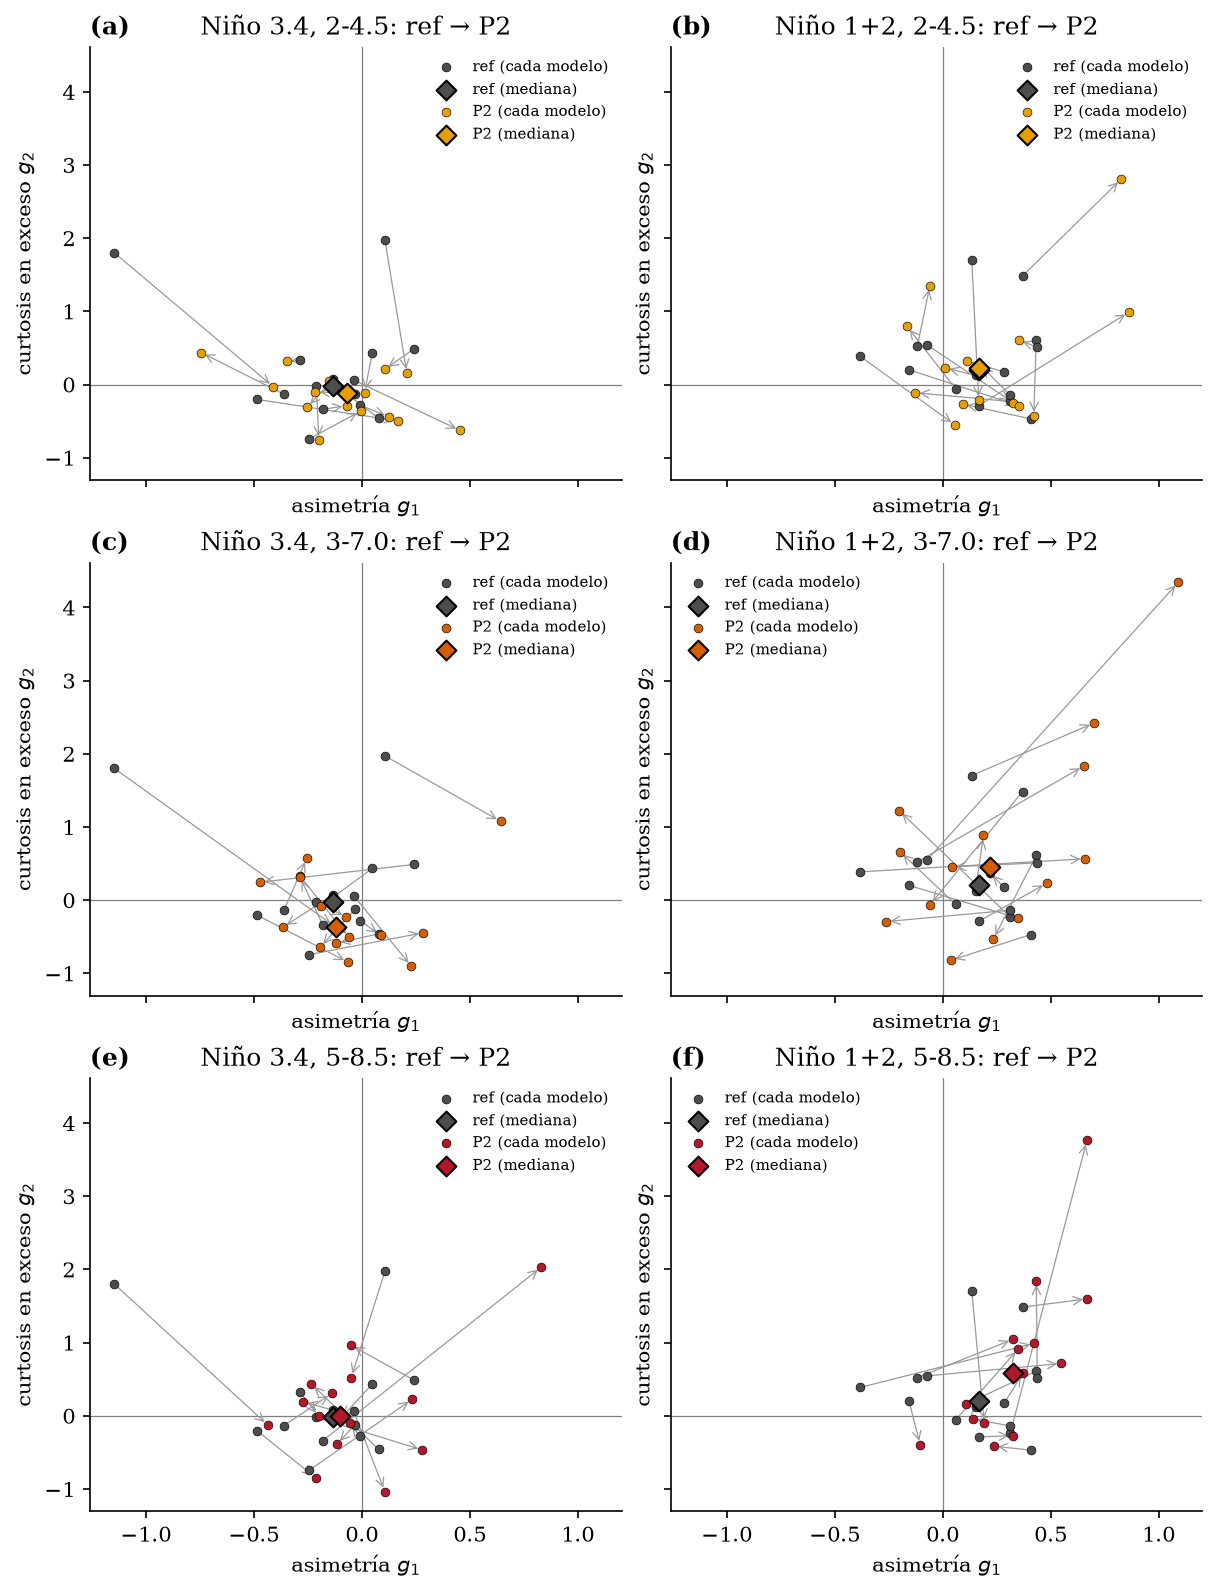
\includegraphics[width=0.9\textwidth]{figuras/e3_A05_asimetria_curtosis.png}
\caption[Asimetría y curtosis de la anomalía, ref y P2.]{Asimetría ($g_1$) y curtosis en exceso ($g_2$) de la anomalía mensual sin tendencia, en ref (gris) y P2 (color), para Niño~3.4 (izquierda) y Niño~1+2 (derecha) y cada escenario (filas). Flechas: cambio de cada modelo; rombos: medianas de los 15 modelos.}
\label{fig:a_asimetria}
\end{figure}

\subsection{Series de los índices hasta 2100}

Con bases móviles (Figura~\ref{fig:a_indices}) la mediana de los modelos es casi plana, porque los Niños de unos modelos se cancelan con las Niñas de otros; lo informativo es la serie de un modelo (AWI-CM-1-1-MR), que muestra eventos individuales, y el ancho de la banda. Con base fija (Figura~\ref{fig:a_fijos}) el índice sube con el calentamiento y a fin de siglo queda por encima del umbral de 0.5\,°C casi todo el tiempo, que es lo que cuantifica la Figura~\ref{fig:umbral}.

\begin{figure}[htbp]
\centering
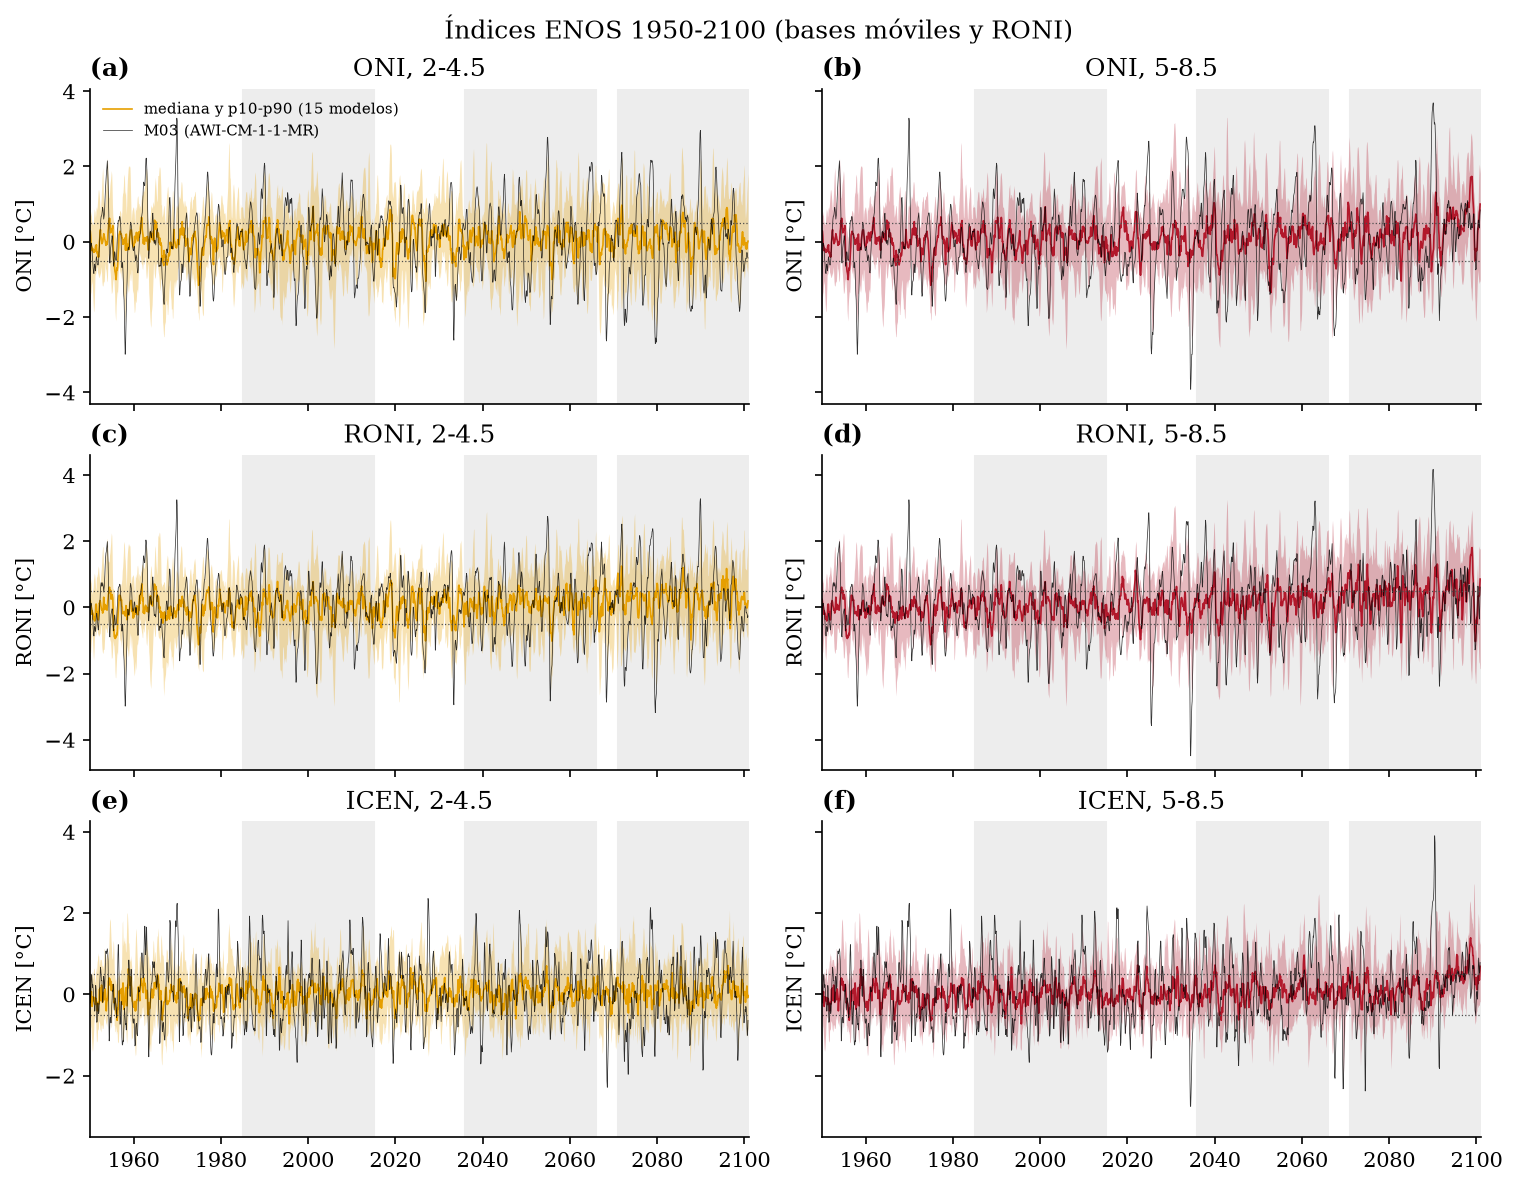
\includegraphics[width=\textwidth]{figuras/e3_A06_indices_envolvente.png}
\caption[Índices ONI, RONI e ICEN, 1950--2100.]{Índices ONI, RONI e ICEN (filas), 1950--2100, por escenario (columnas). Color: mediana y percentiles 10--90 de los 15 modelos; línea negra: AWI-CM-1-1-MR (M03); líneas punteadas: $\pm0.5$\,°C. Franjas grises: ref, P1 y P2.}
\label{fig:a_indices}
\end{figure}

\begin{figure}[htbp]
\centering
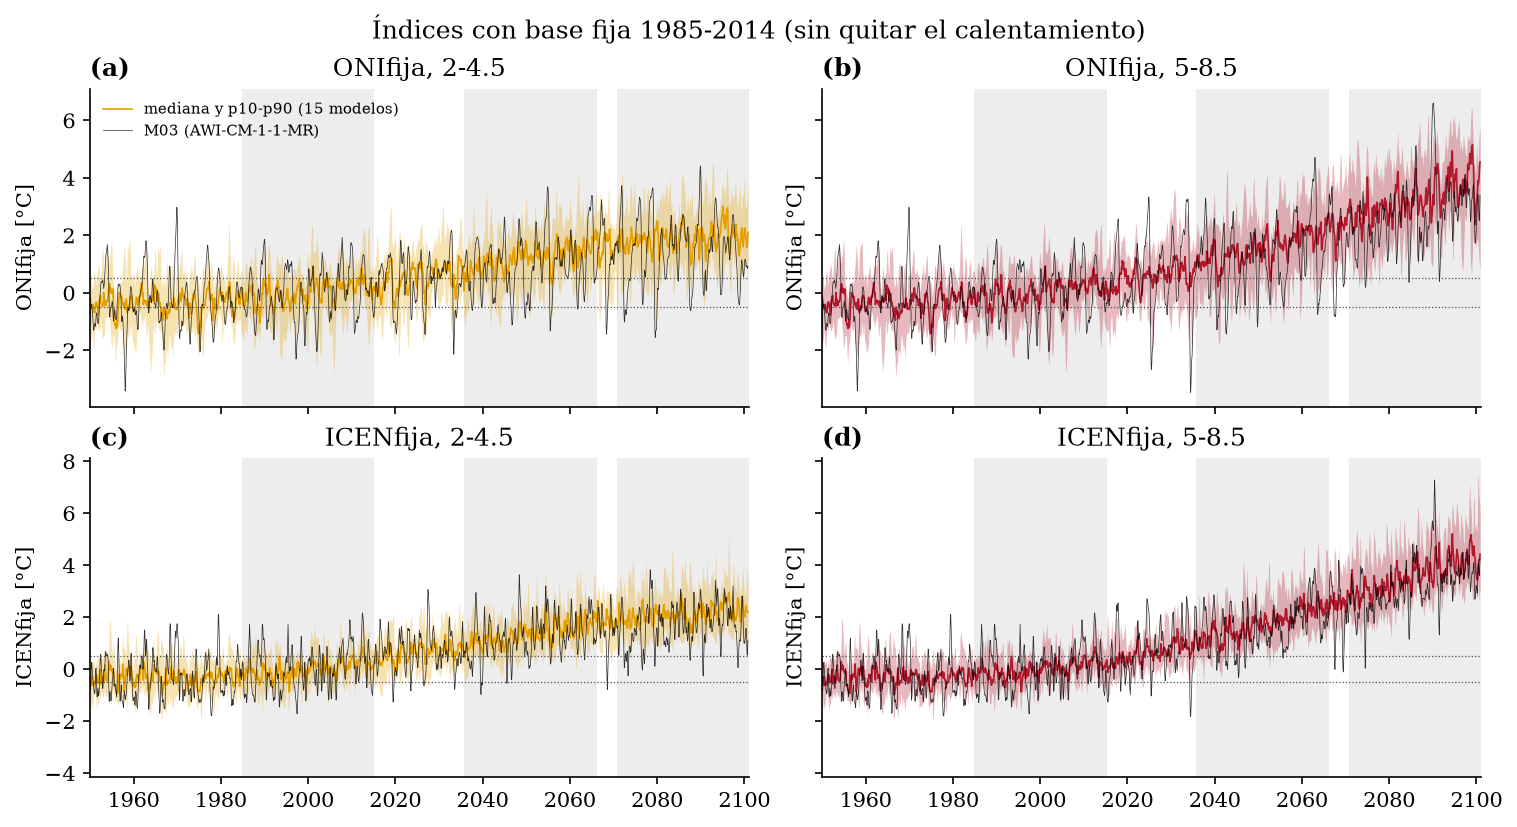
\includegraphics[width=\textwidth]{figuras/e3_A07_indices_base_fija.png}
\caption[Índices con base fija 1985--2014, 1950--2100.]{Índices con base fija 1985--2014 (ONIfija e ICENfija), sin retirar el calentamiento. Formato como en la Figura~\ref{fig:a_indices}.}
\label{fig:a_fijos}
\end{figure}

\subsection{Tipo de evento: costero, extendido y central}

\textbf{Qué se hace:} se cruzan los eventos del ICEN y del ONI del mismo modelo. Un Niño solo en la costa (ICEN sin ONI) es \emph{costero}, como el de 2017; uno en ambas cajas, \emph{extendido}, como el de 1997--1998; uno solo en el Pacífico central (ONI sin ICEN), \emph{central}. \textbf{Por qué:} los impactos en el Perú dependen de dónde se concentra el calentamiento, no solo de cuántos eventos hay.

\noindent\textbf{Definición formal.} Dos eventos de índices distintos son el mismo episodio si sus intervalos [inicio, fin] se superponen al menos un mes. La fracción costera es $f_c = n_{\mathrm{costero}}/n_{\mathrm{ICEN}}$; la clasificación sigue, en su forma operativa más simple, la distinción entre los regímenes de calentamiento del Pacífico oriental y central \citep{takahashi2011}.

En la Figura~\ref{fig:tipo}, los extendidos dominan en todos los periodos y son los que más aumentan: de 8 a 10 cada 30 años en P2 con SSP3-7.0 y SSP5-8.5. Los costeros se mantienen en 1 a 2 cada 30 años. La fracción de eventos del ICEN que son costeros baja en la mediana, de 0.22 a 0.08--0.11 en P2, pero sin acuerdo entre modelos.

\begin{figure}[htbp]
\centering
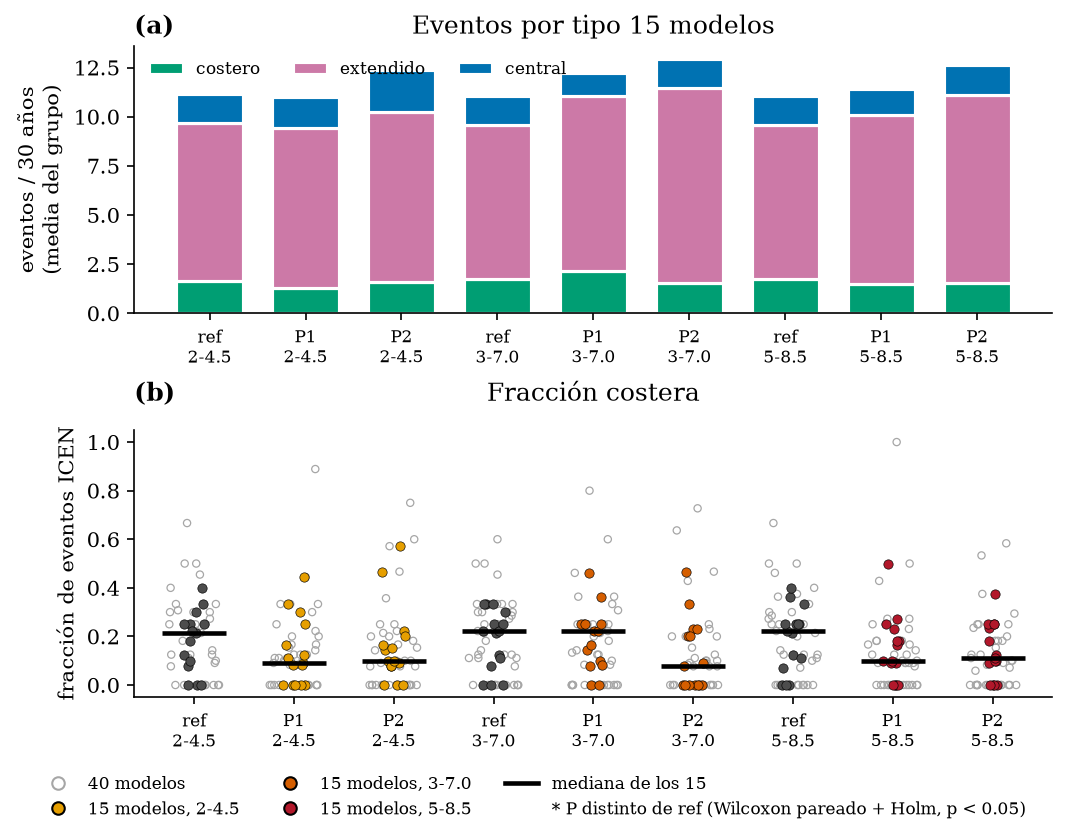
\includegraphics[width=\textwidth]{figuras/e3_A08_tipo_eventos.png}
\caption[Eventos cálidos por tipo: costero, extendido y central.]{(a) Eventos por 30 años según su tipo, media de los 15 modelos: costero (ICEN sin ONI), extendido (ICEN y ONI superpuestos) y central (ONI sin ICEN). (b) Fracción de eventos del ICEN que son costeros, por modelo; formato como en la Figura~\ref{fig:caracteristicas}.}
\label{fig:tipo}
\end{figure}

\subsection{Espectro de potencia}
\label{sec:espectro}

\textbf{Dato:} la serie mensual de un índice (ONI, RONI o ICEN) en un periodo de 30 años. \textbf{Qué hace:} descompone la serie en oscilaciones de distinta duración (cada 2 años, cada 3, cada 5\ldots) y mide cuánta de la variabilidad aporta cada una, igual que un ecualizador de música separa graves y agudos. El resultado es una curva con un pico en el ritmo dominante; en el ENOS observado está entre 3 y 5 años.

\textbf{Por qué:} $\sigma$ dice qué tan intensos son los eventos, pero no cada cuánto ocurren. Si el pico se mueve hacia periodos más cortos, los Niños se harían más seguidos.

\textbf{Cómo se hace (método de Welch):} un espectro calculado con una sola serie es muy ruidoso. Por eso el periodo se corta en 3 tramos de 15 años que se solapan a la mitad, se calcula el espectro de cada uno y se promedian. Aun así, el espectro de un solo modelo sigue siendo ruidoso, y solo se interpreta el del conjunto.

\textbf{Dos resúmenes:} el \emph{periodo del pico} (la oscilación más fuerte entre 1.5 y 10 años) y la \emph{fracción de la variabilidad en la banda del ENOS} (2 a 7 años).

\noindent\textbf{Definición formal.} Método de \citet{welch1967}: la serie $x$ se divide en $K$ segmentos $x_k$ de $L$ meses con 50\,\% de solapamiento; a cada uno se le retira su tendencia lineal y se le aplica una ventana de Hann $w$, y
\begin{equation}
\label{eq:welch}
\hat P(f) = \frac{1}{K}\sum_{k=1}^{K} \frac{\big|\sum_{t} w_t\,x_{k,t}\,e^{-2\pi i f t/f_s}\big|^2}{f_s \sum_t w_t^2}, \qquad f_s = 12~\text{año}^{-1}.
\end{equation}
Con $L = 180$ meses se obtienen $K = 3$ segmentos que cubren los 360 meses. Los 256 meses de la figura del espectro del Entregable~2 sirven para 115 años de registro, pero en 30 años dejarían un solo segmento y fuera de él los últimos 104 meses. Con $K = 3$ y ventana de Hann, cada frecuencia tiene unos 6 grados de libertad. La resolución es $1/15$ ciclos por año, con periodos resueltos en la banda del ENOS de 7.5, 5, 3.75, 3, 2.5 y 2.14 años, por lo que el periodo del pico es discreto. Las métricas son $1/f^{*}$, con $f^{*} = \arg\max \hat P$ en $1.5 \le 1/f \le 10$ años, y $\sum_{2 \le 1/f \le 7} \hat P \,/\, \sum_f \hat P$.

El ritmo dominante del ENOS en los modelos está entre 3 y 4 años en la referencia. En el futuro el pico tiende a correrse levemente hacia periodos más cortos (de 3.75 a 3 años en la mediana de varios casos), lo que sugeriría eventos algo más seguidos, pero con solo seis frecuencias resueltas en la banda del ENOS y bandas entre modelos muy anchas, el cambio no es robusto.

\begin{figure}[htbp]
\centering
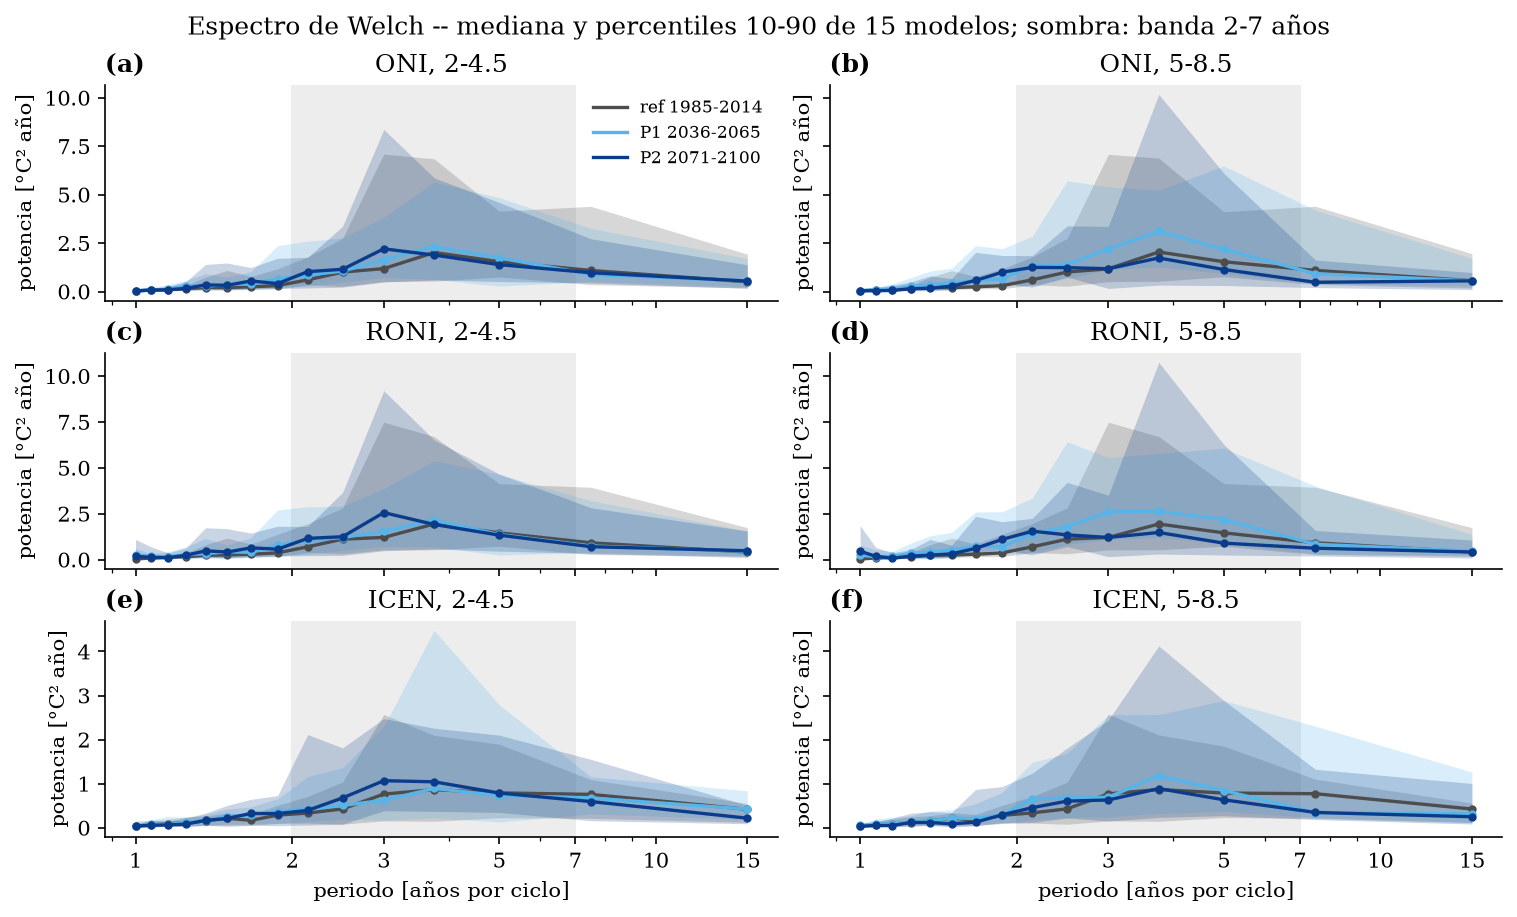
\includegraphics[width=\textwidth]{figuras/e3_A09_espectro.png}
\caption[Espectro de potencia de los índices.]{Espectro de Welch de ONI, RONI e ICEN (filas), por escenario (columnas). Gris: ref; celeste: P1; azul oscuro: P2. Línea: mediana de los 15 modelos; sombra: percentiles 10--90; franja gris: banda del ENOS, 2--7 años. Eje horizontal: periodo en años por ciclo, en escala logarítmica.}
\label{fig:a_espectro}
\end{figure}

\subsection{Sensibilidad al conjunto de modelos}

La Figura~\ref{fig:a_sensibilidad} repite las medianas del Cuadro~\ref{tab:sintesis} para P2 con los cuatro conjuntos. Las medianas cambian poco al pasar de 15 a 40, 11 o 7 modelos: por ejemplo, el calentamiento de Niño~1+2 con SSP5-8.5 es de $+3.6$\,°C con 15, 40 y 11 modelos y de $+3.2$\,°C con 7. La selección del Entregable~2 no altera la señal proyectada; su valor está en descartar modelos que no representan bien los eventos actuales. Con 7 modelos ningún cambio puede salir significativo tras Holm, por eso sus marcadores están vacíos; con 11 solo lo son los cambios en que coinciden casi todos los modelos (Sección~\ref{sec:multimodelo}).

\begin{figure}[htbp]
\centering
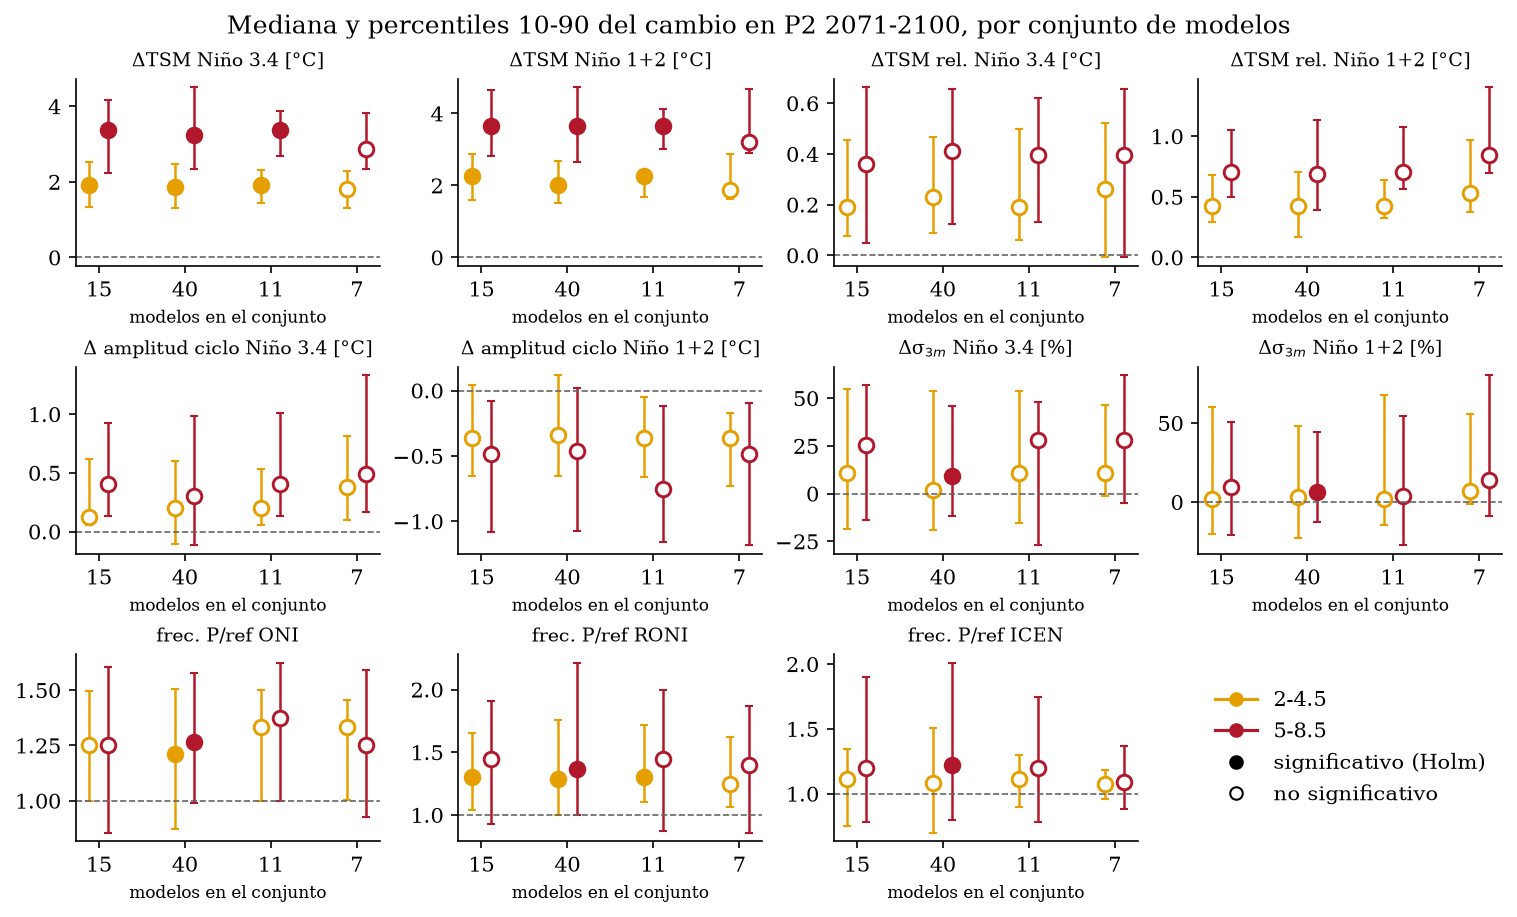
\includegraphics[width=\textwidth]{figuras/e3_A10_sensibilidad_conjuntos.png}
\caption[Sensibilidad del cambio en P2 al conjunto de modelos.]{Mediana (punto) y percentiles 10--90 (barra) del cambio en P2 para cada conjunto de modelos (15, 40, 11 y 7), con SSP2-4.5 (amarillo) y SSP5-8.5 (rojo), los dos extremos del rango de escenarios. Marcador lleno: significativo con Wilcoxon y Holm.}
\label{fig:a_sensibilidad}
\end{figure}

\end{document}
